\documentclass[12pt]{report}

\usepackage[margin=2.0cm]{geometry}
\usepackage[defaultlines=3,all]{nowidow}
\usepackage{graphicx}
\usepackage{amsmath}
\usepackage{epstopdf}
\usepackage{float}
\usepackage{hyperref}

\usepackage{color}
\usepackage[table,xcdraw]{xcolor}
\usepackage{listings}
\usepackage{caption}
\DeclareCaptionFont{white}{\color{white}}
\DeclareCaptionFormat{listing}{\colorbox{gray}{\parbox{\linewidth}{#3}}}
\captionsetup[lstlisting]{format=listing,labelfont=white,textfont=white}

\setlength\parskip{0.5em}
\newtheorem{theorem}{Theorem}

\title{Implementing the beta machine on a Terasic DE10 SoC+FPGA development board}
\author{Master's thesis carried out to obtain the degree of Master of Science\\ in Electrical 
Engineering by Polet Quentin\\ \\ University of Liège - School of Engineering and Computer Science}
\date{Academic year 2020-2021}

\begin{document}

\pagenumbering{gobble}
\vspace*{3cm}
\begin{figure}[h!]
    \centering
    
\includegraphics{res/uliege-logo-couleurs-300.jpg}
\end{figure}
{\let\newpage\relax\maketitle}
\vspace*{\fill}

\newpage

\pagenumbering{arabic}

\chapter*{Acknowledgements}

I am grateful to all those who helped and supported me during this work. In particular professors 
Fontaine Pascal and Mathy Laurent who were very regular in their follow-up by participating with me 
in regular meetings. In addition to that, they were available to answer all my questions during the 
whole duration of this work, which was very reassuring and helpful. I would like to thank Professor 
Fontaine in particular for his very careful review of this work and for the many pertinent 
suggestions that resulted from it. But also for putting me in touch with people who could guide me 
on certain choices for this work.

These two people are Nadel Alexander who is a research scientist at Intel Israel and Gyuszi 
Suto a principal engineer at Intel Oregon. I thank them greatly for the time they devoted to me through 
several emails and a video conference meeting during which I could present my work and discuss with 
them. They specifically helped me in the choices of how I could 
improve the confidence one could have in a Central Processing Unit (CPU) such as the one developed in this work.

I would also like to thank Mormont Romain, a PhD student at the University of Liège in machine learning
who provided an assembler software that outputs beta machine code. He also took 
the time to explain me how it works and how to use it by mail. One last person directly involved in 
this work is Schnackers Gauderic, a physics engineer who took the time to try out the system 
designed in this work by programming a 2D video game on it. I thank him for this and for his friendship.

Finally, I could not end my thanks without thinking of all my family and friends who have always been 
very supportive and who knew how to entertain me when I wanted to work too much.

\chapter*{Introduction}

Although some liberties have been taken at the end of the work, the main objective of this master thesis
is to provide a laboratory tool for the computation structures course INFO0012-2 at the University of Liège. Indeed, the professors of 
the course needed a replica of the beta machine, an Harvard architecture based CPU that is learned
throughout the course. This machine had to be physically implemented so that the students could 
really take it in hand rather than using simulations. In order to design it in hardware, it was 
decided to work on an Field Programmable Gate Array (FPGA), a Cyclone V from Altera to be precise. In fact, everything was done on a 
development board, the DE10-Nano from Terasic. This allows to focus almost exclusively on the logic and 
structural implementation rather than on all the electrical details intrinsic to such 
implementations.

This document therefore starts with a first chapter containing an enumeration of the different 
functionalities of this board as well as a description of the generalities about FPGAs. A quick 
comparison with other similar technologies is also made. Then, an overview of the two parts of the 
FPGA, starting with the programmable logic followed by the ARM processor part is done. The existing 
interconnection between these two parts is also described afterward. The last part of this chapter 
is a comparison between the different memories available on the board and on the FPGA.

After introducing the hardware, an introduction to the FPGA development flow is 
given. In this chapter, a brief discussion on the different specific tools used throughout this work 
is made. The specificities of the programming language used, i.e., Verilog, are also presented. The
chapter finally closes with a discussion on the compilation flow.

Now that the groundwork has been laid, the core of the matter can be addressed. This is why the 
third chapter contains a description of the beta machine. In this description, the reader is 
made aware of the dimensioning of the machine: the word size, the endianness of the machine, its 
instruction set, etc. Following this, the implementation of the CPU on FPGA is presented in detail. 
The IO unit which provides access to several IOs of the DE10-nano board to the CPU is also
described in this chapter.

At this stage, the specifications are fulfilled for the hardware part of this master thesis. That
said, it would have been a shame to deliver this machine without any interface other than what is 
possible using the IO unit. This is why the following chapter details the implementation of a 
graphics accelerator which will be abusively called GPU (Graphics Processing Unit). The HDMI controller and the protocols 
allowing its use are introduced beforehand. The clock unit (CLKU) is also presented.

Chapter 5 covers the design of the Memory Access Unit (MAU) which gives access to the memories of 
the beta machine from the ARM processor. The description of the Control Unit (CTRLU) allowing the 
startup and shutdown of the machine from the ARM processor is given here. The communication 
protocol common to both units is first presented before detailing the implementations. 

In order to provide easy access to the machine, an operating system must be installed on the ARM 
part of the FPGA. Chapter 6 discusses the choices made at this level.

Finally, a chapter is dedicated to the different tools developed to facilitate the access and the 
programming of the machine by the users. This last chapter also lists different demonstrations 
programmed in assembly language that serve as proof of concept. The assembly libraries written for 
this work are also briefly presented.

% PF: when you first use an acronym, define it
% QP: Ok
% PF: do not forget acknowledgements
% QP: Job done!

\chapter{Overview of the hardware}

\section{Features of the DE10-Nano development board}

% PF some are not grammatically correct sentences below
% QP OK
Numerous devices are made available to the user on the DE10-Nano development board. Some of them are very 
interesting for this work. The Cyclone V FPGA is one of them. It includes a configurable part (the programmable 
logic) and an ARM processor (A in Figure \ref{fig:de10/de10_features}). The Cyclone V is
basically the main component of the system as almost everything on the board is driven by it. It is
also where all the hardware designed in the work resides. The 1GB DDR3 RAM (B) which is used 
by the ARM side of the FPGA. An ethernet port (C) which can be
useful to connect to the ARM processor from any external environment. For instance, SSH can be used
to connect to it if the installed system can handle it. Then there are the SD card reader and the SD 
card (D, on the other side of the board). The SD card consists in the mass storage of this board. The
one used offers 8GB of memory. Another important component is the HDMI output (E) that can be used
from the programmable logic side of the Cyclone V. Other less important devices, mainly IOs are 
available: General Purpose Input / Output pins (GPIOs), LEDs, buttons and switches. All of these 
devices are discussed at some point in this report. The ones that are not listed (such as the Inertial
Measurement Unit, IMU) haven't been used.

\begin{figure}[H]
    \centering
    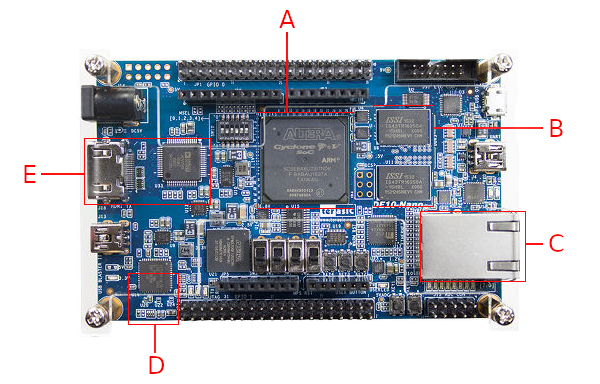
\includegraphics[scale=0.5]{Chapter1-Hardware/res/de10_nano.png}
    \caption{DE10 Nano development board main features.}
    \label{fig:de10/de10_features}
\end{figure}

\section{Programmable logic devices}

Field Programmable Gate Arrays (FPGAs) are a type of Programmable Logic Device (PLD) which are, as 
the name suggests, programmable logic circuits. Programmable means that the user can choose which 
circuitry is implemented in these devices.  As seen later in this chapter, some of 
these devices are very versatile! They can implement almost any kind of digital circuit.

PLDs come in different flavors but follow a similar pattern for most types. In fact, they almost all 
are composed of an AND array and an OR array that are both programmable or not. Here, a discussion 
of the different types of PLDs and their evolution is made before describing FPGAs. The advantages 
and disadvantages of these technologies are also detailed.
% PF will be made to arrive at : this is heavy, try to rephrase the whole sentence (show the ... is not that nice either)
% QP OK

\subsection{ROM based PLDs}

This first type is very simple, as shown in Figure \ref{fig:fpga/pld_rom_external}. In fact, the 
circuit, which can only be combinatorial, is simulated by a ROM. Each address corresponds to 
an input of the circuit and each word in memory to an output of the circuit. The ROM therefore 
simply contains the truth table of the logic circuit to be implemented.

\begin{figure}[H]
    \centering
    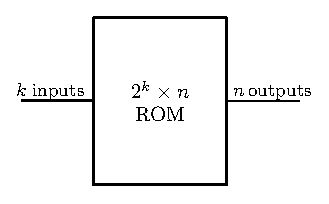
\includegraphics[scale=1.2]{Chapter1-Hardware/res/pld_rom_external}
    \caption{An external view of ROM based PLDs.}
    \label{fig:fpga/pld_rom_external}
\end{figure}

The inside of a $2^2 \times 4$ ROM can be seen as a 2-to-4 decoder followed with a 4-by-4 OR gates 
array, as shown in Figure \ref{fig:fpga/pld_rom_internal}, where the connections in the array are configurable. They can be opened or closed while
programming the device. The decoder can be interpreted as the AND gates array here. Thus, the
AND gates array is fixed and the OR gates array is programmable for this kind of devices.

In the example of Figure \ref{fig:fpga/pld_rom_internal}, the array is represented by a grid. All horizontal lines represent a 1-bit signal
that can be connected to an OR gate. The signal is connected if a red x is present at the connection
point. In the figure, each OR gate can thus be connected to at most 4 decoder bits. As can be seen, 
the OR gates array is here programmed to describe the truth tables of these 
boolean equations

\begin{equation*}
    \begin{cases}
        A_0& = I_0 \cdot \bar{I_1} \\
        A_1& = \bar{I_1} \\
        A_2& = 0 \\
        A_3& = \bar{I_0} \cdot I_1
    \end{cases}
\end{equation*}

% PF shouldn't you say also to what the horizontal lines correspond?
% QP It is done line 62

Obviously, real devices contain a lot more signals and gates to be cost effective and useful. 
As stated previously, the ROM PLDs can only represent combinatorial circuits. There is no register
or feedback loop in the circuits that are described with this technology.

\begin{figure}[H]
    \centering
    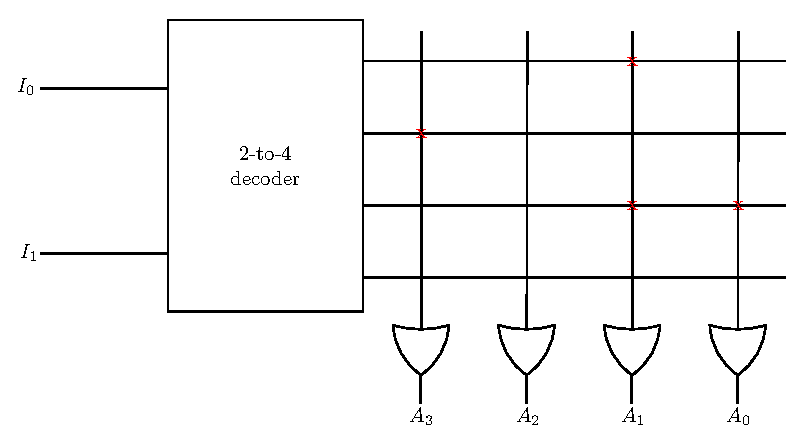
\includegraphics[scale=0.8]{Chapter1-Hardware/res/pld_rom_internal}
    \caption{An internal view of ROM based PLDs.}
    \label{fig:fpga/pld_rom_internal}
\end{figure}

\subsection{PAL and PLA}

The Programmable Array Logic (PAL) and Programmable Logic Array (PLA) devices differ from the ROM 
based PLDs since they both have a programmable AND gates array. However, only the PLAs have both AND and
OR gates arrays that are programmable, the OR array is not programmable for PALs. The PLAs are thus 
the most flexible devices of the three.
As expected, this flexibility makes them also more complex and complicated to program. The outputs
of these devices can often be complemented through programming too. It should also be noticed
that both the inputs and the inverted inputs are directly available in the arrays here, as illustrated on
Figure \ref{fig:fpga/pld_pla_internal}. 
% PF I do not understand the previous sentence
% QP I removed the sentence

\begin{figure}[H]
    \centering
    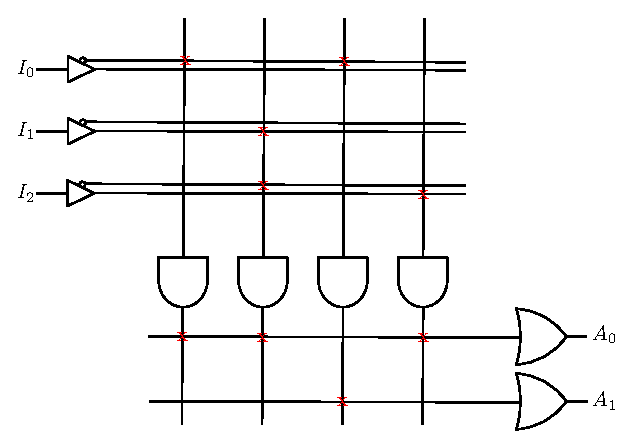
\includegraphics[scale=0.8]{Chapter1-Hardware/res/pld_pla}
    \caption{An internal view of PLAs.}
    \label{fig:fpga/pld_pla_internal}
\end{figure}

\subsection{Programming methods}

This section contains a brief discussion of the various usual programming techniques.
% PF do not use a sarcastic tone as in the above sentence ;-).  Use short sentences, straight to the point.
% QP OK
 
Initially, these devices were mainly programmable in two ways. The first was to use fuses and 
anti-fuses at each interconnection. The user then had to apply destructive currents to the right 
places for the fuses to open the connections and the anti-fuses to close them. The second method was 
to leave it to the user to complete the IC design. One would then make a mask to select which 
interconnects to open and close during a lithography process. To provide some examples, the fuse 
methods are used in PROMs and 
masks for ROM based PLDs. Both of these programming methods make the devices non-erasable, which at 
the same time makes them non-reprogrammable. However, they are both non-volatile which can be an 
advantage when the user don't want any boot latency at startup, as no programming phase is needed at boot
time.

Later, other programming techniques were developed following the emergence of transistors. Indeed, 
these transistors are placed at the interconnections and controlled by their gate with the help of 
a bit kept in a memory. The memory can then be programmed to define the behaviour of the connections 
without them being frozen forever. As the memory is usually SRAM, the devices become reprogrammable
but still volatile. Other technologies have subsequently made it possible to have non-volatile 
memory in addition to memory by using, for example, floating gate transistors. These two types of 
interconnections are usually configured by applying a high current to set or reset the memory state. 

\section{The case of FPGAs}

Now that PLDs and programming methods are introduced, it is time to get to the 
core of the matter with a description of FPGAs.  This section aims to be general 
enough to cover the operation of a large number of FPGAs. More details specific to the FPGA actually used in this work are given in the next 
section.

%PF fascinating yet complex devices: is that usually contradictory?  Try to improve
% QP OK
FPGAs have three main programmable levels. These 
three levels are discussed in turn, starting with the programmable logic blocks, then the 
programmable interconnect and finally the programmable I/Os. 

\subsection{Programmable logic blocks}

Programmable blocks are present in very large numbers in modern FPGAs (usually tens to hundreds of 
thousands). They are the basic elements of the circuits implemented on FPGAs. Due to their 
architecture, which can be seen in Figure \ref{fig:fpga/fpga_block}, they allow both combinatorial 
and sequential circuits to be implemented. 

\begin{figure}[H]
    \centering
    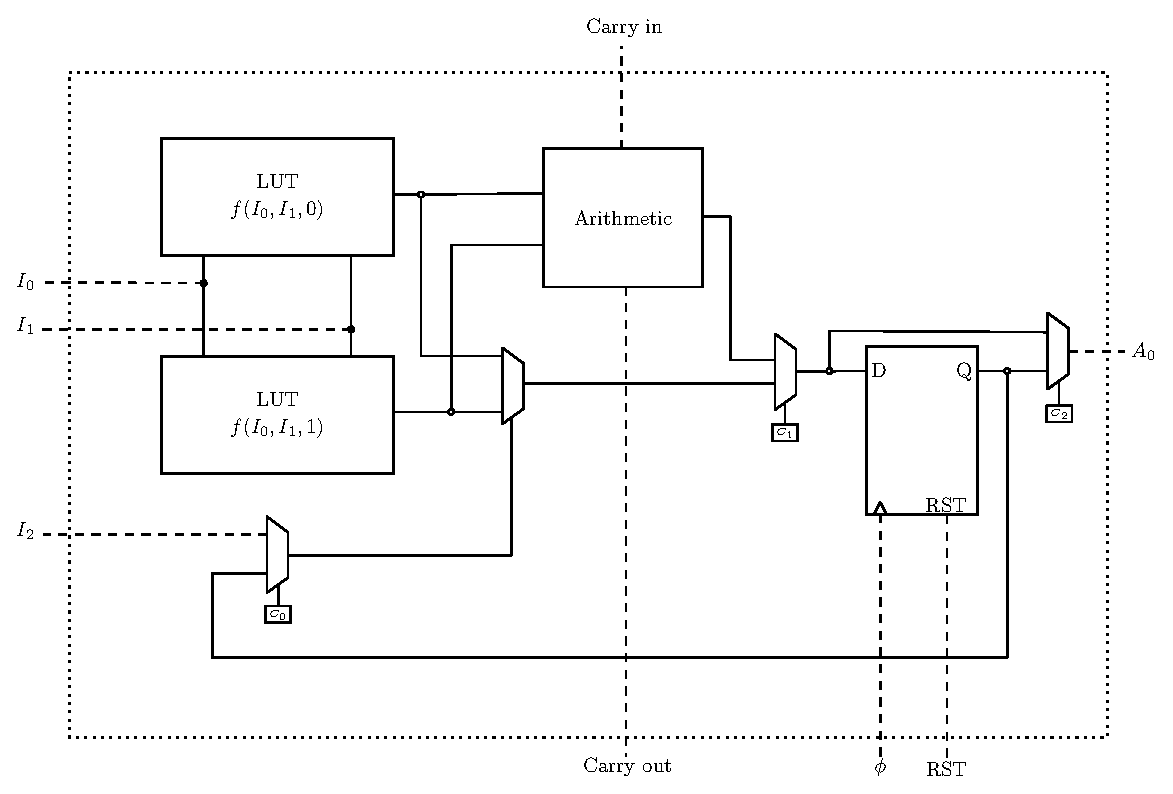
\includegraphics[scale=0.8]{Chapter1-Hardware/res/fpga_block}
    \caption{An FPGA programmable logic block.}
    \label{fig:fpga/fpga_block}
\end{figure}

The combinatorial part of the circuits is implemented using a LookUp Table (LUT). The truth table is 
simply stored in this LUT as for the ROM PLDs but the bits are now stored in SRAM. If one LUT is 
not sufficient, the logic function can be implemented in several LUTs connected at the output by a 
multiplexer that is controlled by the remaining inputs. This is made fully valid by Shannon's 
expansion theorem. 

\begin{theorem}
    Any boolean function $f(x_1, x_2, ..., x_n)$ can be expressed as 
    \begin{equation*}
        f(x_1, x_2, ..., x_n) = x_n \cdot f(x_1, x_2, ..., x_{n - 1}, 1) + \bar{x_n} \cdot 
        f(x_1, x_2, ..., x_{n - 1}, 0)
    \end{equation*}
\end{theorem}

As shown in Figure \ref{fig:fpga/fpga_block}, the blocks also have an arithmetic sub-block and a 
register. Having this arithmetic block in each single programmable block greatly increases the 
efficiency of the FPGAs and reduces the latency of the blocks, even if most of the time these circuits are 
simple carry adders. Fixed hardware is always faster than programmable one as they are better 
optimized. In addition to the programmable LUTs, other configuration bits are available to control
the behaviour of the multiplexers: $C_1$, $C_2$ and $C_3$ allowing respectively to add a feedback 
loop to the block, to select the result of the boolean function or that of the arithmetic sub-block 
and to make the output of the block registered or not.

In brief, these blocks are the heart of the FPGA. All their features and configuration bits allow 
them to describe almost any kind of digital circuit in an efficient way.

\subsection{Non-programmable blocks}

Other non-programmable or less programmable blocks are also available within FPGAs. They are divided 
into two main groups: memories and utilities. Memories are simply blocks that can store data. A 
specific discussion of these memory blocks is made in a later section. On the utility side, 
there can be a wide variety of blocks: multipliers, PLLs, DSPs and even whole CPUs. In short, 
enough to make FPGAs even more powerful!

\subsection{Programmable interconnect}

Programmable blocks are very versatile and efficient, but they need to be connected to each other to 
make large circuits. As can be seen in Figure \ref{fig:fpga/fpga_interconnect}, the blocks are 
positioned on a grid and the interconnection passes around them. 

\begin{figure}[H]
    \centering
    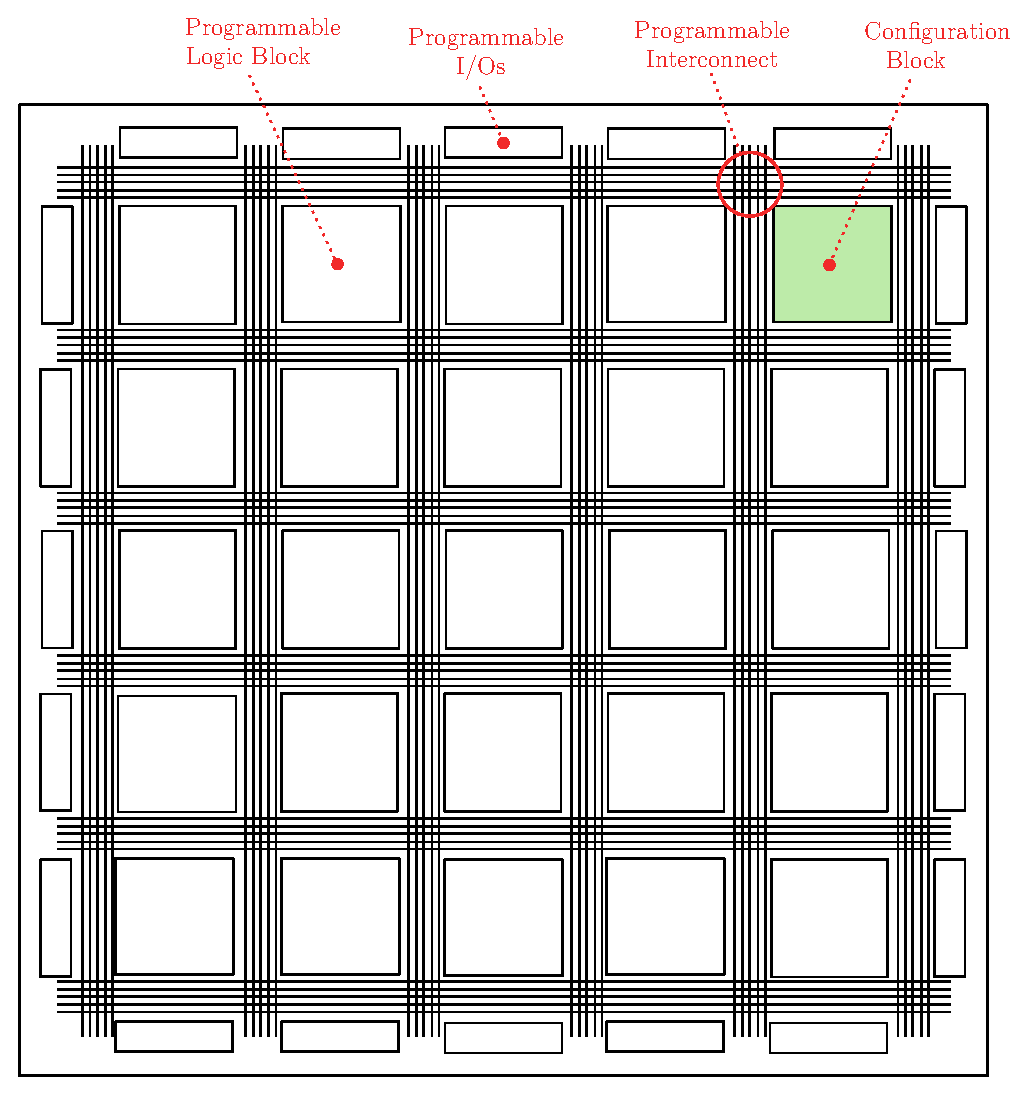
\includegraphics[scale=0.6]{Chapter1-Hardware/res/fpga_interconnect}
    \caption{High level view of an FPGA.}
    \label{fig:fpga/fpga_interconnect}
\end{figure}

For this purpose, there is the programmable interconnection that allows the signals to be routed 
from one block to another. To do this, configurable switches are placed at the crossings of the 
tracks. However, everything must be connected, whether the blocks are close or distant. As this 
cannot be done directly without causing problems in terms of time and power constraints, several 
hierarchical connection levels are present. However, in order to keep the explanations simple, it 
is considered here that there is only one level. It should also be noted that each switch adds 
latency to the signal, so the interconnection is optimised to limit the number of switches between 
blocks. 

In addition to this configurable interconnection, there are also tracks to bring global signals 
everywhere. Among these signals are the clock, the resets, ... On a more local level, some signals 
are also shared between the blocks. These include, for example, the carry signals of the arithmetic 
sub-blocks.

\subsection{Programmable I/Os}

Now that almost the entire interior of the FPGA has been described, all that remains is to connect 
it to the outside. This is why there are these I/O pins all around the FPGA in Figure 
\ref{fig:fpga/fpga_interconnect}. These as well as the other parts of the FPGA are also 
configurable. As it is desirable for the FPGA to adapt to a wide variety of external hardware, these 
pins can be configured to the standard used. They can also be used as input, output, bi-directional, 
differential pairs, ... In short, they allow a large number of configurations so that the designed 
circuit can be adapted and coupled with a maximum of other circuits.

\subsection{Programming the FPGA}

%PF never use Programmation 
%QP OK, my bad

Due to their complexity, the configuration circuitry of the FPGA is just as complex. For this 
reason, few details are provided in this section. That said, it should be noted that part of 
the FPGA is assigned to this function. This block takes care of configuring all the 
configuration bits in the relevant memories. However, since the memories holding the configuration 
within the FPGA are volatile, it is often necessary to couple a non-volatile memory to the 
FPGA to retain its configuration. The configuration therefore has to be re-configured each 
time the FPGA is rebooted, which can create some latency. It is also important to note that the 
memory holding the configuration must be relatively large, as the number of configuration bits is 
very large. More details on compiling designs and configuring FPGAs in practice are given in a 
later section.

This closes the theoretical discussion on FPGAs. As already said, FPGAs are extremely 
powerful and versatile. This enables them to describe a large number of circuits and to adapt to
many existing circuits. Another advantage is that they are massively parallel due to their 
structure. Despite all these 
advantages, FPGAs still have some drawbacks. One of them is cost. Some FPGAs can cost several 
thousand euros. The complexity and difficulty of access is another problem for designers, the 
datasheets are numerous and extremely long, the tools are also numerous and not always easy to use. 
Electrical power requirements and start-up latency are also two other factors that must be taken 
into account when a user chooses an FPGA for circuit development. Nothing is perfect, not even 
FPGAs.

\section{Inside Cyclone V}

\subsection{Programmable logic side}

In the Cyclone V, things are even a little more evolved than previously explained but it is still quite 
accessible. In fact, the programmable logic blocks is replaced here by Logic Array Blocks (LAB) 
which are themselves made up of ten Adaptive Logic Modules (ALMs) which are the equivalent of 
the programmable logic blocks studied previously. A high level view of the LAB units is given in
Figure \ref{fig:cyc5/lab}. In the LAB, the different ALMs, the inputs and outputs of the LAB, can be 
interconnected at the user's convenience.

\begin{figure}[H]
    \centering
    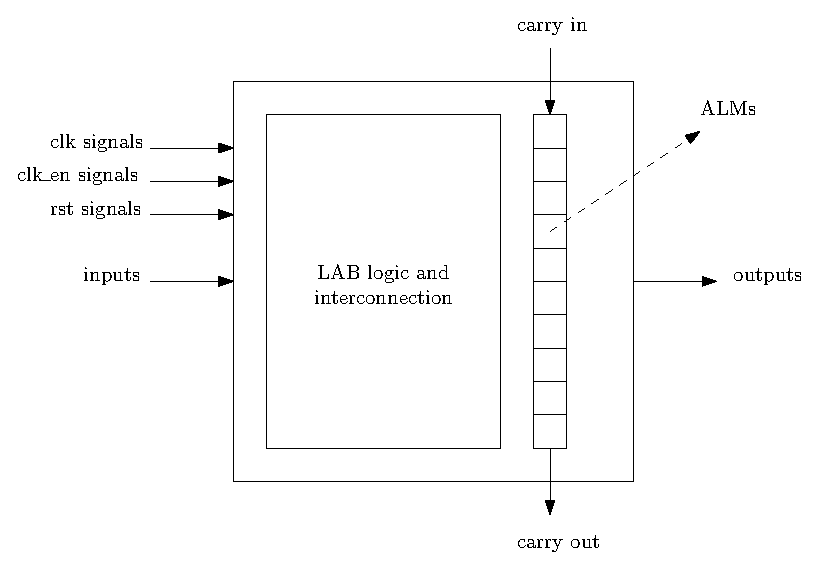
\includegraphics[scale=0.8]{Chapter1-Hardware/res/lab_block.eps}
    \caption{High level view of a LAB unit.}
    \label{fig:cyc5/lab}
\end{figure}

There is also another type of LAB, the Memory LAB (MLAB) which allows to describe SRAM. They can 
store up to 640 bits and represent 25\% of all the LABs present on the Cyclone V. These MLABs do not 
have memory instead of
% do you mean besides the the ALMs?
% QP yes
the ten ALMs, they also have the ten ALMs and all the logic necessary 
to use them. They are a superset of LAB somehow.

These LABs (and MLABs) are placed in the FPGA fabric in an array as explained in the previous 
section. However, it should be noted that the array is not symmetrical with respect 
to the vertical and horizontal connections at the local level (this part was not detailed 
previously). Indeed, the horizontal connections aim to connect the blocks close to each other by 
ensuring a high speed of operation. These are the inputs and outputs that are mainly linked to it. 
The columns, although they are also fast, are mainly used for carry signals. At the local level, a 
LAB can have control over 30 ALMs: its own ten, and the ten of its two horizontal neighbors. This
allows to build very complex logic in a restricted space. Of course, a more global interconnection 
allows all LABs to be connected together. There are many more details about the internal 
connections of the LABs that could be discussed, but these are not explained in this report.

Concerning the ALMs, as just said, they are very similar to the Logic Array Blocks of 
the previous section. The main differences are that they accept more inputs, up to eight. The 
internal arithmetic block is in fact two separate adders, and four registers are provided in each ALM. 
Depending on their configuration (set during the programming phase), ALMs are adapted to 
specialize in a functionality to make the circuits more efficient (for example more entries, an 
optimization for arithmetic, shared arithmetic with an input of the adder that is fed by an input 
of the ALM, ...). 

\subsubsection*{Other blocks}

The LAB blocks are very customizable and extremely numerous on the Cyclone 5. However, there are 
several other types of blocks that are worth listing and briefly explaining. The overall structure 
of the Cyclone V FPGA is shown in Figure \ref{fig:cyc5/structure}.

\begin{figure}[H]
    \centering
    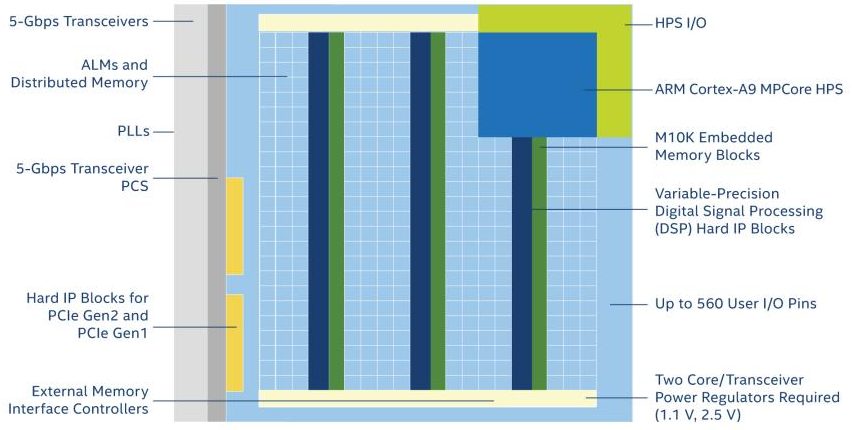
\includegraphics[scale=0.6]{Chapter1-Hardware/res/cycv_structure.PNG}
    \caption{Overall structure 
    of the Cyclone V FPGA \cite{cyc_web}.}
    \label{fig:cyc5/structure}
\end{figure}

The largest block visible on the diagram is the one at the top right which represents the entire ARM
system, this block is discussed in the next section. Then one can see many dark 
green columns that designate the M10K memories. These memories are the main source of on-chip 
storage.  A sub-section of this chapter is dedicated to the memories, and they are studied in more 
detail there. The PLLs are also visible in the light gray band on the left. PLLs allow to 
generate clocks at a given frequency from a reference clock. Again, this unit is studied later. 
Another element present in large quantities is represented by the dark blue columns. It is the 
Digital Signal Processing (DSP) Hard IP Blocks. These blocks have a multitude of functions. Indeed, 
they provide arithmetic units of addition, subtraction and multiplication, allow the implementation 
of filters, ... In this work, they are only used to perform operations such as addition, 
subtraction and multiplication in the Arithmetic Logic Unit (ALU). It should be noted that using 
these DSPs is much more advantageous than using ALMs. Indeed, the arithmetic circuits of the DSPs 
are "hard-made" which means that they have no programmable interconnection logic in their internal 
circuits, so the delays are much smaller and their architecture is totally optimized. For the user, 
this allows him to use higher clock frequencies than he would have been able with circuits designed
with ALMs. Other units are available but are not discussed.

\subsection{ARM processor side}

Inside the FPGA, a 32bits ARM processor, often named Hard Processor System (HPS), is integrated. It is a Cortex A9. No bare-metal programming 
is done on this processor. It is used as an interface to access the beta machine. Indeed, 
an operating system has been installed on it and utilities have been developed so that the use of 
the architecture developed in this work is easily accessible. Discussions about the operating system 
and the tools are done at the end of this document. For the moment no description is made. That 
said, it was important to mention it in this part of the report as it constitutes a large part of 
the Cyclone V hardware. Furthermore, it was necessary to introduce it before starting the next two 
sections.

\subsection{Cyclone V interconnect}

As just mentioned in the previous section, the ARM processor serves as the user interface. 
Therefore, one needs a way to communicate between the ARM processor and the programmable logic of the 
FPGA (which will now be refered to as FPGA although the ARM processor is also part of the FPGA). 

In fact, there are bridges between the two sides. These bridges are the link between the two parts 
and can be used for communication. Each of these bridges has a specific purpose, it is not just the 
same one put several times in parallel. The first and most basic bridge is the Lightweight HPS-to-FPGA 
bridge. This one is designed for small transactions that are ponctual, the user should avoid for example 
streaming data on this channel (even if nothing prevents it). The limitation in size comes from the 
fact that the data bus of this bridge is only 32 bits wide. As the name of the bridge indicates, it 
is unidirectional and goes from the HPS to the FPGA. Then come two more interesting bridges: the 
FPGA-to-HPS Bridge and the HPS-to-FPGA Bridge. The directions of these two buses are obvious. What 
is less obvious is their size. On the HPS side, their dimension is fixed at 64 bits, but on the FPGA 
side, they have the great advantage of being able to be configured to 32, 64 or 128 bits. 
These bridges are ideal for large data transfers. Finally, there are the FPGA-to-SDRAM bridges which 
allow six masters on the FPGA side to have a non cached and non coherent access to the RAM memory. 
This is discussed in the next section in more detail. These different bridges all allow several
masters on one side to be connected to multiple slaves on the other. The selection of the 
slaves is done by byte aligned addresses. The address space is therefore the only thing limiting the 
number of slaves on a bridge. In order to better visualize the interconnection, a diagram is provided 
in Figure \ref{fig:cyc5/interconnect}. In this work, only the HPS-to-FPGA bridges are used.
% PF use present as long as it is possible: it makes things simpler
% QP OK

\begin{figure}[H]
    \centering
    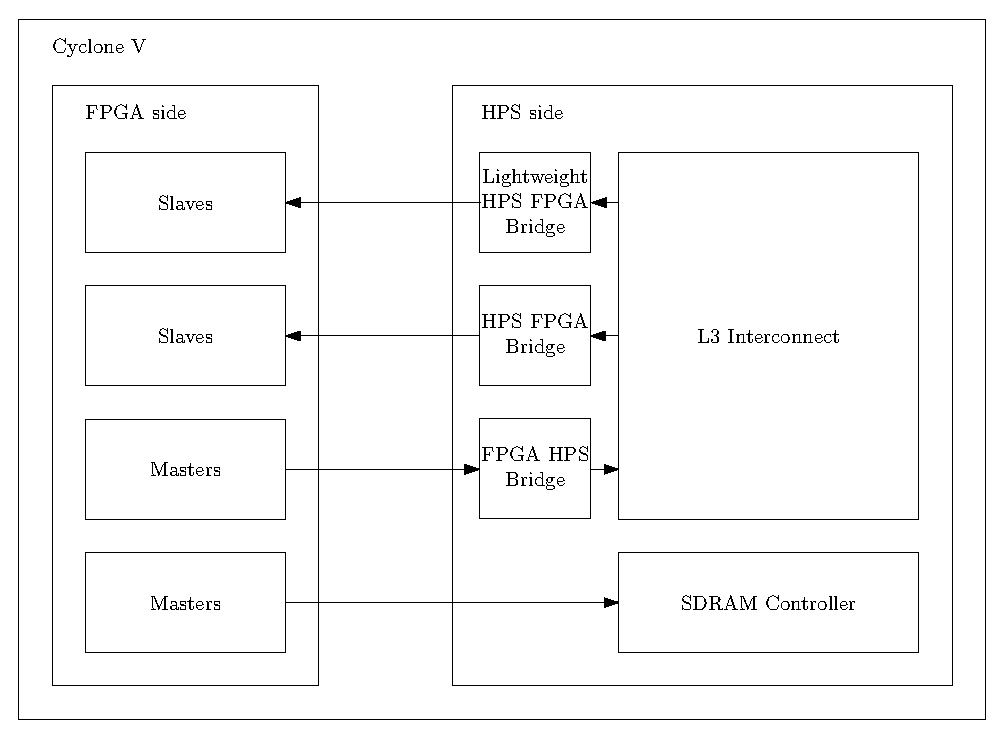
\includegraphics[scale=0.6]{Chapter1-Hardware/res/cycv_interconnect}
    \caption{Interconnect bridges.}
    \label{fig:cyc5/interconnect}
\end{figure}

In Figure \ref{fig:cyc5/address_space} the address mappings from different viewpoints are shown. For 
the two buses going from the HPS to the FPGA, it is the MPU column (Memory Protection Unit, the unit 
that protects memory accesses on ARM architectures) that is of interest. One can see that the address 
space is much larger for the HPS-FPGA
% PF is there a reason to use lower case here?
% QP No, modified!
bridge than for its lightweight equivalent. These addresses 
are those to which the slaves on the FPGA side are associated and therefore those to which one
has to send the transactions from the ARM processor in order to communicate with these slaves. 
The protocol is of course studied in this document but this is done when the transactions 
between the two parts are discussed.

\begin{figure}[H]
    \centering
    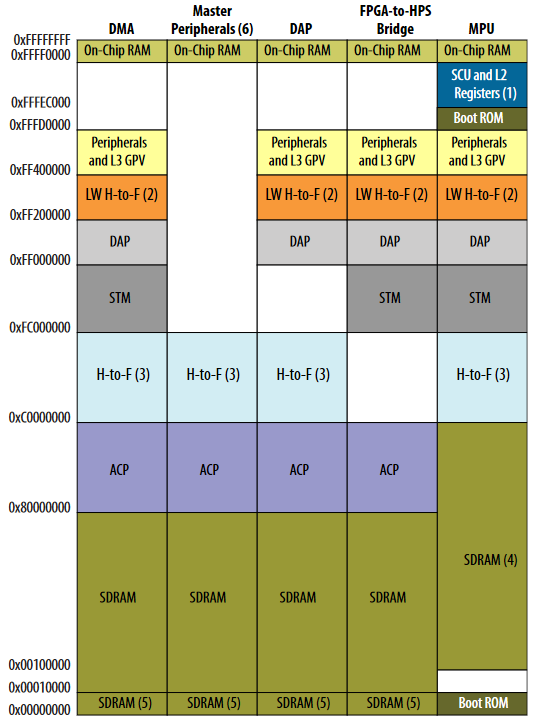
\includegraphics[scale=0.6]{Chapter1-Hardware/res/hps_address_space.PNG}
    \caption{Address maps for system interconnect masters \cite{hps}.}
    \label{fig:cyc5/address_space}
\end{figure}

\section{On-board and on-chip memories comparison}

As seen in the previous sections, several types of memories are available. Directly on the board 
there is the SD card storage and DDR3 RAM memory. On the Cyclone V there are also two types of memory 
which are MLAB units and M10K blocks. Each memory has its own features. Since both the beta 
machine and the ARM system require memory, it is interesting to consider the use of these different 
memories, compare them and finally make a choice.

Let's start with the simplest, the ARM processor. In fact, on this side no choice is left to the 
user. The DDR3 memory serves as the main memory and the SD card as the secondary memory for 
non-volatile storage. 

Concerning the Beta machine, the choice is less obvious.  Which memory to choose to store 
instructions and data, as main memory?  Given the nature of the SD card memory, it can immediately be 
ruled out of the possible choices. What about the other memories?
% PF I do not like much the questions in the text, but since you do not use them much, it is quite OK
% QP These are the only ones of this work so I decided not to modify this paragraph.

\subsection{DDR3 memory}

The DDR3 memory offers 1GB 
shareable between the ARM processor and the FPGA,
% PF maybe not already talk about the beta machine, but just FPGA
% QP OK
which is really huge. However, an almost 
direct access to this memory is only possible if the access is done in a non-caching and 
non-coherent way with respect to the ARM processor caches. Another possibility is to use the ACP 
ID mapper which ensures a cached and coherent access (using the L2 cache). The two access paths 
are identified in Figure \ref{fig:de10/ddr3}. The problem with these two accesses is that they are 
not instantaneous, the writes and reads do not take the same number of cycles and the number of 
cycles is not unitary. To use these memories, it is therefore necessary to either slow down the 
whole system on the FPGA or to have a cache memory on the FPGA with faster memory next to it. In 
addition to this, in the first case (direct access) it is necessary to configure the operating 
system on the ARM processor to ensure that it never accesses the part of memory reserved for the
FPGA system and in the second case (with the ACP) it is necessary to configure the ACP 
correctly so that its operation is as expected. In both cases this means modifying the kernel of the 
operating system, which is not necessarily simple. For these two reasons: the delays and the 
necessary modifications at the kernel level, this memory has not been chosen. However, it could be 
a very interesting modification of the system built in this work to provide more memory to it.

\begin{figure}[H]
    \centering
    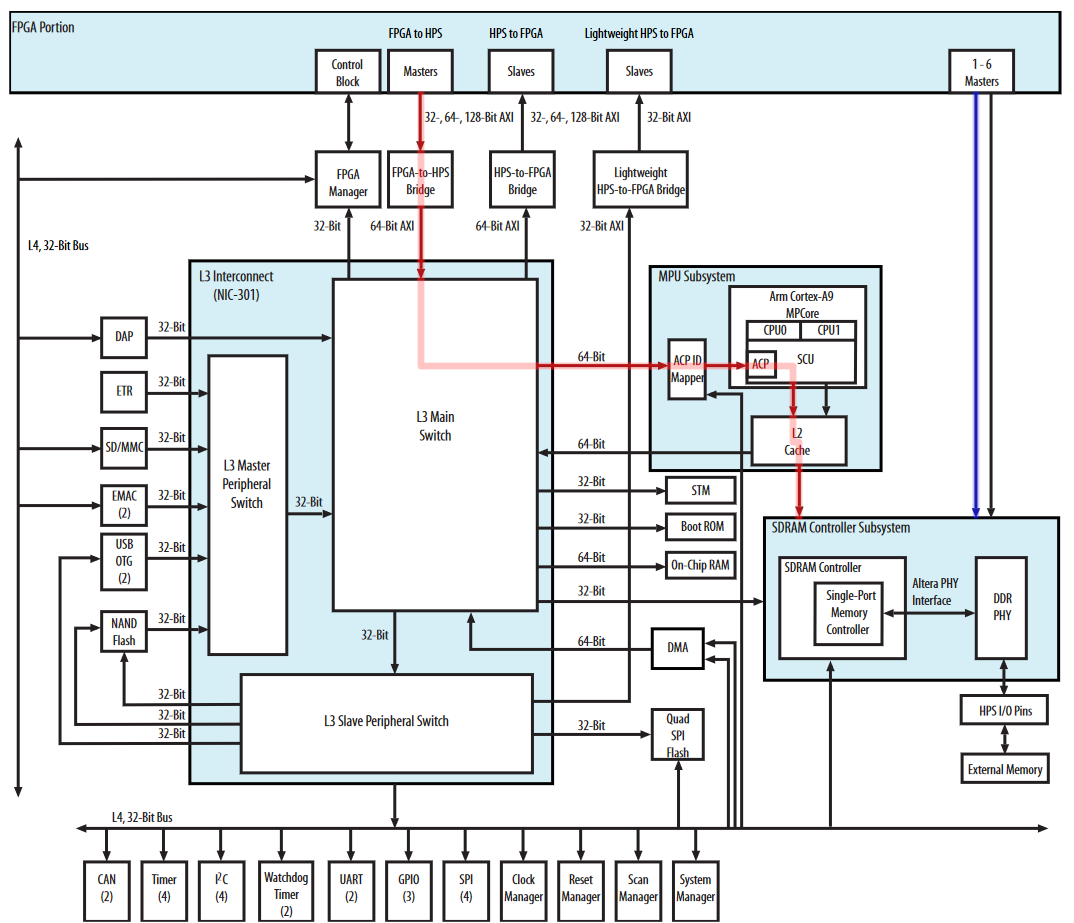
\includegraphics[scale=0.4]{Chapter1-Hardware/res/de10_DDR3.PNG}
    \caption{DDR3 accesses from the FPGA. Red path uses the ACP and blue path is a direct access
    to the memory controler \cite{hps}.}
    \label{fig:de10/ddr3}
\end{figure}

\subsection{M10K and MLAB memories}

What about the M10K and MLAB memories? These two memories are directly present on the FPGA, which
 means that they can be read and written in one clock cycle. Moreover, they are not used by the 
 ARM processor, which avoids having to take care of the coherence of the caches. How to choose 
 between these two memories? The first difference is the amount of memory available. Indeed, there
 are 553 M10K memory blocks in the Cyclone V SE A6
% do you mean: there are 533 M10K modules in the Cylcone V SE A6 ?  See later for the same clumsy construction
% QP OK
 used in this work. As a M10K memory 
 contains 10Kb, the whole of these blocks represents a little more than 5Mb which is already very 
 large for a machine like the beta machine. There are also 994 MLABs blocks containing 640 bits each, 
 as seen previously. This makes a total of a little more than 600kb. 
 However, there are three reasons why the choice is made for the M10K rather than the MLABs. 
 The first reason is that MLABs use up programmable logic; the more MLAB memory is used the less 
 custom logic can be added to the FPGA, up to a loss of 25\% if all memory is used. The second is 
 that the datasheet advises to use these memories in cases where shallow and large memories are 
 needed. This is because it is complicated to create large memories locally with MLABs. Last 
 but not least, MLABs do not provide dual-port access, which is a huge handicap because it is 
 necessary to duplicate the memories if the user wants this kind of access. As the choice of M10Ks 
 seems to be the most suitable for this work, it is decided to use this source of memory.  To keep things simple, 
 hybrid systems are avoided.  Another difference between MLABs and M10Ks is that 
 MLABs have no problem running at frequencies up to 420 MHz while M10Ks do not go beyond 315 MHz. 
 However, the system of this work does not exceed a 50 MHz clock frequency, so frequencies are of little concern here.

\chapter{Hardware design flow on FPGA}

Now that the reader is aware of the internal structure of FPGAs, the design flow on these FPGAs can 
be discussed. Indeed, a series of more or less compulsory steps are required to carry out the 
design of an embedded system on FPGA. This chapter is dedicated to the description of this 
design flow and the tools used to carry it out. All the tools that are discussed in this chapter are
part of a super-tool named Quartus. Quartus is the main software used for the development on Intel 
FPGA. In fact, it is a kind of IDE for hardware development. It interfaces many tools together to
ease the work of the users.

\section{Design flow}

The very first step is of course to choose an FPGA, once this is done, one must start by assigning 
the inputs and outputs of the FPGA. This step is named I/O Planing in Figure \ref{fig:flow/design_flow}.

\begin{figure}[ht]
    \centering
    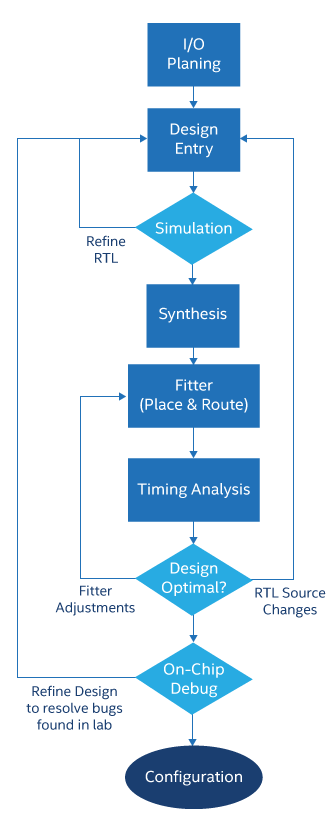
\includegraphics[scale=0.5]{Chapter2-FPGA_Flow/res/blockdiagram-quartus-flow.png}
    \caption{Intel FPGA design flow on Quartus \cite{quartus}.}
    \label{fig:flow/design_flow}
\end{figure}

\subsection{I/O Planning}

% PF generally, in computer science, the user is female: her design
% not important.  I would use "her/his"
% QP OK, there are to many him/his to modify so I didn't do it
During this I/O Planing step, the user has to choose which input or output of his design goes to 
which physical input or output of the FPGA. It is also during this step that the types of I/Os, the 
standards they should use etc. are set. In the context of this work, this step could be skipped. 
Indeed, the manufacturer of the DE10-Nano board provides with its board a Quartus project 
containing the definition of the I/Os in order to correspond to what is present on the board. 
This greatly simplifies the task and avoids digging through all the datasheets of the different
components of the board to find out how to set up all the IOs.

\subsection{Design Entry}

In this step, the user defines the different logical entities that are needed to build up the 
desired circuit. A logical entity or a module is simply a sub-circuit with a given interface, an
example is shown later in this section.

All this is done in a so-called hardware description language. There is no need for special tools 
here, a simple text editor will do. However, Quartus contains an editor that can be used for this 
purpose. Concerning the languages, there is a multitude of choices. But there are three frequently used 
languages. These are VHDL, Verilog and System Verilog. VHDL is a high level language that is highly typed.
Verilog and System Verilog are weakly typed and lower level. For example, in VHDL it is 
frequent to work directly on data-structures, complex types that can quickly hide the logic of an 
architecture. In Verilog and System Verilog, few types are provided and the hardware architect does 
regularly work with registers and words in which the bits are assignable one by one. Since System 
Verilog is a newer language and not always (correctly) supported by the tools, it was decided to use 
Verilog for this work. 

It should be noted that these languages, although similar to software programming languages, do not 
work in the same way. Indeed, in a Verilog file for example, one defines so-called modules. 
A module has inputs and outputs. Each input and output can either be defined as a wire, 
which means that this I/O have no specific functionality, it just serves as a connection, or 
as a reg, which means that this I/O is registered. A register is therefore placed at this I/O. 

Inside the module, the developer then defines how these inputs and outputs are linked. Here again, 
two possibilities are available to the user. Indeed, it is possible to define circuits that are 
either combinatorial or sequential. For the combinatorial circuits, they can take any input 
(registered or not) and transmit its outputs to non-registered outputs. It is important that the 
output is non-registered because combinatorial circuits are asynchronous, the compiler would not 
understand who is driving the register if it was put directly at the output of a combinatorial 
circuit. The other possibility is to describe sequential circuits. For these, a sensitivity list 
must be chosen. That is to say, signals that have the effect of updating the circuit. In 
general, only the clock is used, and the state of the circuit changes at each clock cycle. Note that
any other signal specified in that list might result in an asynchronous response of the circuit, as
the circuit responses to a clock change and also to a change of this signal. This is useful to
implement asynchronous resets in synchronous circuits. Inputs of sequential circuits can be registered or
not but sequential circuits can only transmit their output to registers. It should be noted that a combinatorial 
circuit and a sequential circuit can be cascaded since sequential circuits accept non-registered 
inputs. This makes it possible to put a combinatorial output on an output register for example, even
though it is impossible with the combinatorial circuit alone. 

At the level of sequential circuits, another subtlety compared to software programming languages 
should be noted. The assignment of registers is done in a blocking way. This means that these 
assignments are only effective at the next clock cycle (or next sensitivity signal update) and 
that all these assignments are made at the same time in parallel. One should not forget that the 
language describes circuits. And so all outputs appear at the same time once the rising or falling 
edge of the clock is perceived. For example assigning $x$ to $a$ and then $a$ to $b$ results in
$a[t]$ containing $x[t - 1]$ and $b[t]$ contains $a[t - 1]$, which might not be obvious for a software
developer.

To better illustrate the above notions, a small example of a module described in
Verilog is given below.  It simply describes an AND logic gate whose output
is registered. The corresponding circuit is shown in Figure
\ref{fig:verilog/register_and}.

{\small
\begin{lstlisting}[language=Verilog, caption=Verilog Registered AND gate example.]
module registered_and(
    clk,
    input0,
    input1,
    output0
);

// clk is defined as an input wire 
input wire clk;   
// input0 is defined as an input wire  
input wire input0;  
// input1 is defined as an input wire
input wire input1; 
// output0 is defined as an output and it is registered
output reg output0; 


// An internal wire is defined
wire and_output;    

// Describes an and gate between input0 and input1
// and put the result on the wire and_output asynchronously
assign and_output = input0 & input1; 

// Sequential circuit that updates at rising edge of clk
always @(posedge(clk)) begin
    // The circuit simply directs the value present on "and_output" at 
    // that moment to the registered output (i.e., it sets the register).
    output0 <= and_output;                      
end

endmodule
\end{lstlisting}}

\begin{figure}[H]
    \centering
    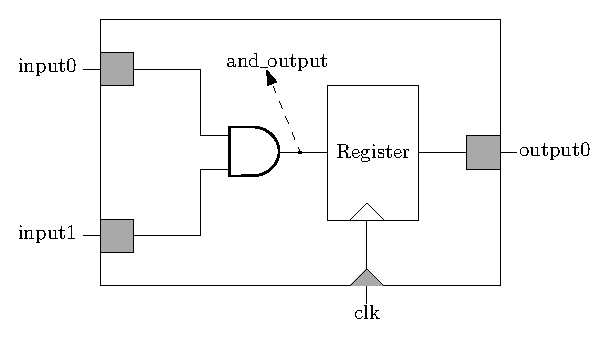
\includegraphics[scale=1.0]{Chapter2-FPGA_Flow/res/register_and}
    \caption{Intel FPGA design flow on Quartus.}
    \label{fig:verilog/register_and}
\end{figure}

Other tools than programming allow to define modules. A particularly useful tool is the IP creation 
Mega Wizard shown in Figure \ref{fig:tools/megawizard}. This tool allows the user to create some common 
blocks such as on-chip RAMs using a graphical interface where one can choose the different options. 
For a RAM the user can choose the word size, the number of words, whether the memory has 
two ports or not, etc. At the end of the configuration, the wizard generates the Verilog file 
describing the module just defined.

\begin{figure}[H]
    \centering
    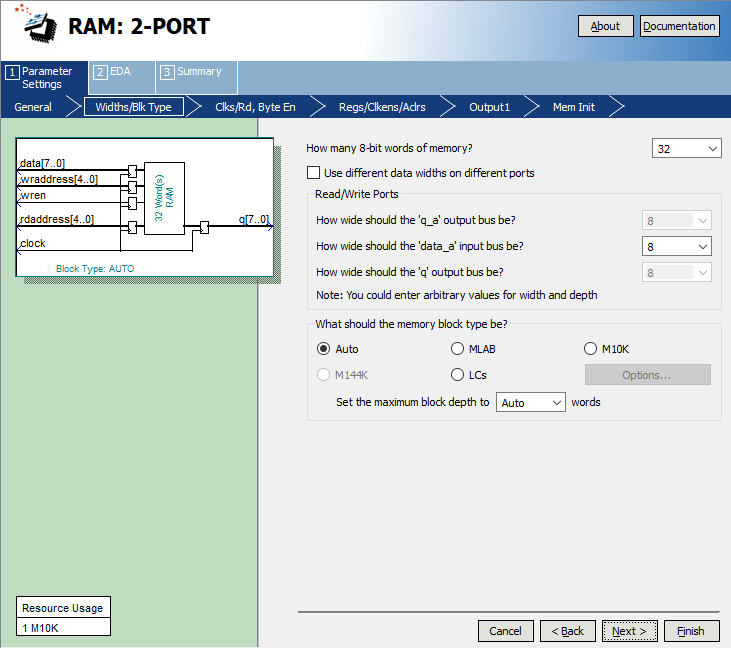
\includegraphics[scale=0.6]{Chapter2-FPGA_Flow/res/megawizard.PNG}
    \caption{IP creation Mega Wizard window.}
    \label{fig:tools/megawizard}
\end{figure}

\subsection{Interconnect Design Entry}

This step is equivalent to the simple design entry, i.e., the goal is to describe the architecture. 
However, as the tool to design the interconnect is specific, a section is dedicated to it. 
As discussed previously the interconnect is the part of the architecture that links the FPGA and the ARM. The 
use of the buses is done through several signals, which can quickly become intricate to 
maintain directly through Verilog files. The specific tool for this, Qsys, allows to link 
the masters and slaves of the FPGA to those of the ARM processor in a graphic interface. In fact,
one can add several slaves or masters in QSys and link them to the desired bridge.  In this 
tool, the address space of each slave has to be specified. Qsys checks if the specified 
addresses are not outside the address space of the master to which they are connected. Figure \ref{fig:tools/qsys} 
shows the interface to the HPS (ARM processor) and the connections to a slave.

In addition to the signals that are useful for communication on the interconnect, others allow interaction 
with the FPGA. This means that these signals are inputs or outputs of the Verilog code that is generated
by QSys. They can thus be connected to other circuits on the FPGA side, contrary to the other
signals shown in QSys. These signals are called exported signals and the user can chose which one
is exported, usually the ones that are not direct links of the interconnect. Once a system is 
described, it only
remains to ask Qsys to generate the system. It then creates all the necessary Verilog files that 
can be used as a single module later in user's Verilog code. This module receives as inputs and 
outputs all the signals that have been exported. To summarize, QSys is a kind of graphical 
programming software.

\begin{figure}[H]
    \centering
    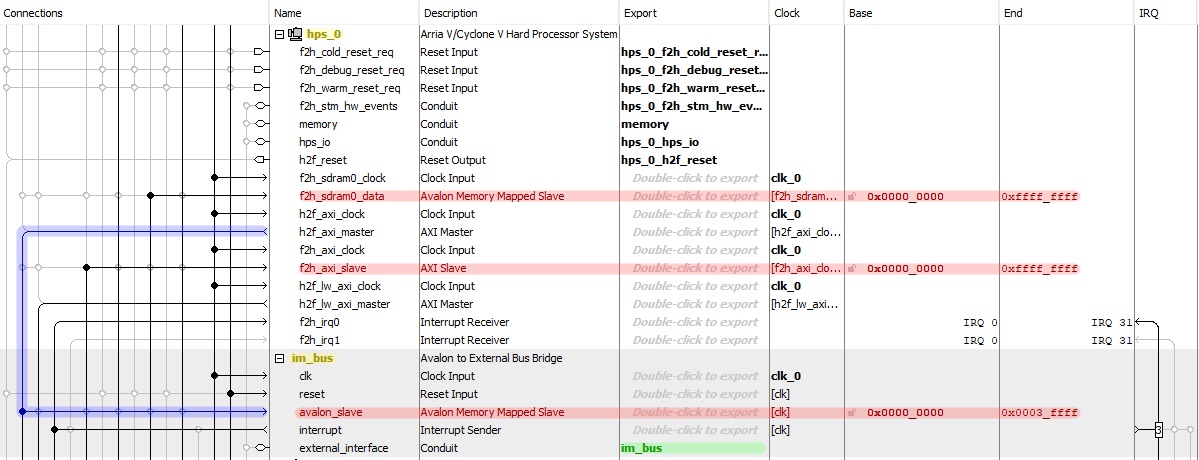
\includegraphics[width=\linewidth]{Chapter2-FPGA_Flow/res/qsys.PNG}
    \caption{QSys window with an HPS named hps\_0 and a slave module named mm\_bus.}
    \label{fig:tools/qsys}
\end{figure}

Figure \ref{fig:tools/qsys} highlights different elements. The two entities present in the system are 
represented in yellow, there is thus the HPS named hps\_0 which is an external representation of the 
ARM processor and an Avalon to External Bus Bridge called im\_bus which makes it possible to make 
the link between a bus of the interconnection and a bus defined by the user on the FPGA. This module 
is discussed again later. In each module, some lines are in red, to denote the 
different slaves of the system. In the base and end columns, it can be seen that these slaves have 
a defined address space. They all start at 0 because they are relative to the starting address of 
the master. In the im\_bus an exported signal is highlighted in green: it is accessible 
from the FPGA. In fact, most of the lines shown in QSys represent several signals describing entities,
bus, ... Finally, a master-slave connection is shown in blue.

% PF I must say that this above section is a bit more abstract to me, most probably because I do not see
% clearly what you are doing with these connections
% QP I added a sentence in paragraph 1 but I don't see how to better explain.

\subsection{Simulation}

Once the different modules of the system have been defined, it can be interesting to simulate some 
of them. This step is not necessarily mandatory but it can save a lot of time if the system is large. 
Indeed, compiling a large system can quickly take several hours, or days.  It is thus beneficial to
conduct verifications before compilation using simulation rather that later on by measurements on the working 
system. 
Sometimes, the simulation is also more practical because it allows to easily generate detailed 
scenarios. To simulating tool used by quartus is Modelsim. In this tool, signals can be fixed 
and tests can be performed. All signals are then displayed so that the user can verify the 
behavior.

\subsection{Synthesis and Fitter}

These two steps are the firsts of the compilation. The compiler transforms the descriptions made
 in Verilog into a logic circuit and then try to fit everything on the target FPGA. It checks that 
 the resources are sufficient for the given design. The whole fitting process is 
 time-constrained. This means that it places the different blocks in such a way that the delays 
 are minimal. After the Synthesis, the user can display the circuit to verify parts of its design
 visually. The tool used for this is the RTL net viewer. An example is given in Figure 
 \ref{fig:tools/rtl}.

 \begin{figure}[H]
    \centering
    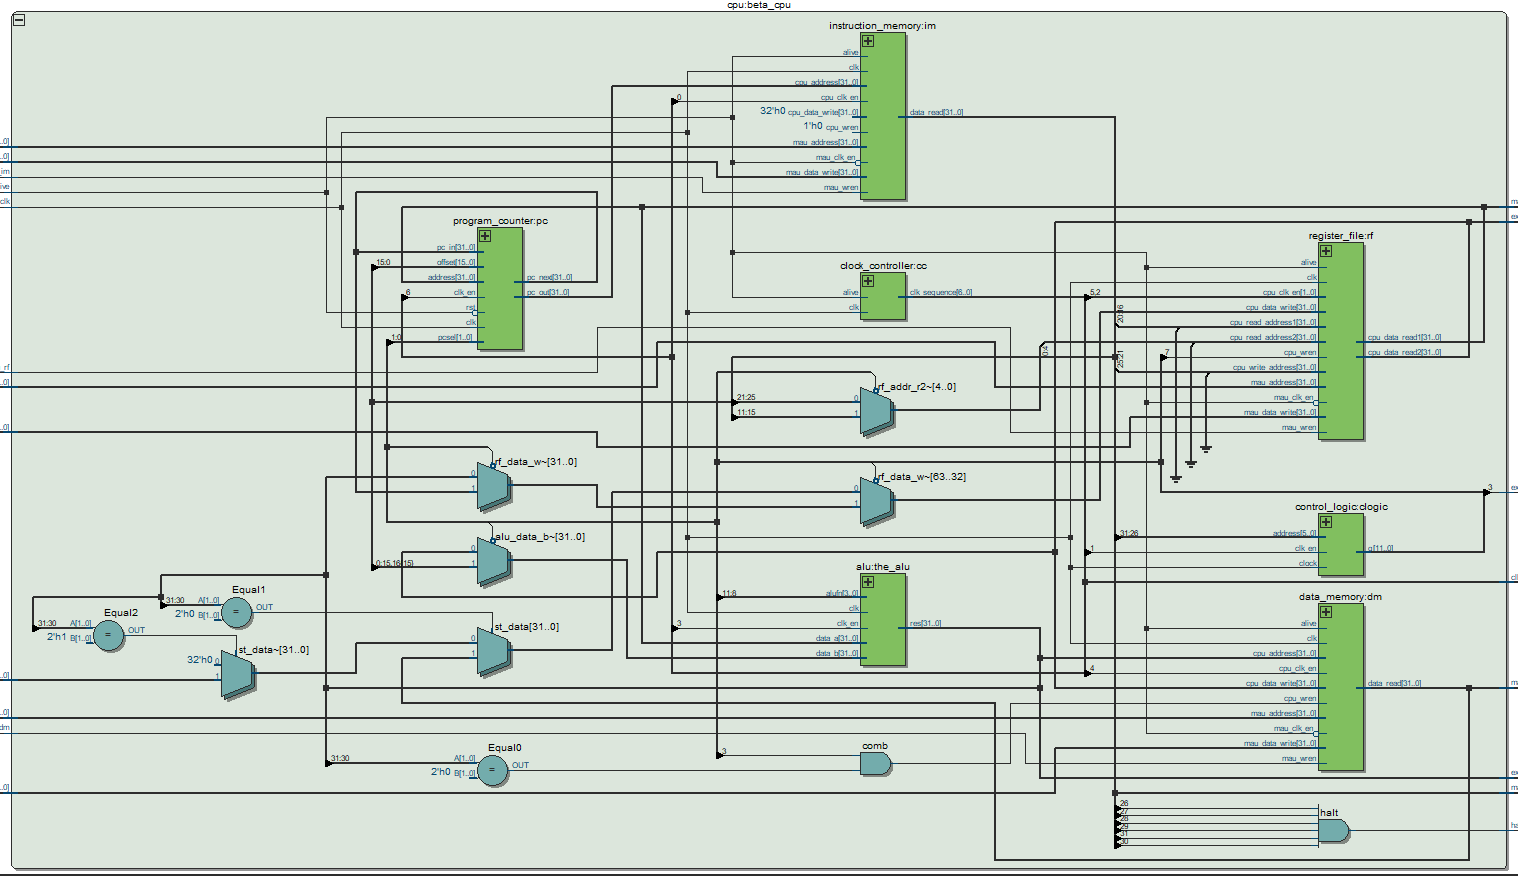
\includegraphics[width=\linewidth]{Chapter2-FPGA_Flow/res/rtl.PNG}
    \caption{The beta machine CPU high level view in RTL viewer.}
    \label{fig:tools/rtl}
\end{figure}

\subsection{Timing Analysis and Design Optimal}

FPGA designs are strongly dictated by time constraints. The purpose of this step is to check if the 
constraints are well respected by the design, after fitting. All this is done by simulation by 
testing the signal propagation delays at different temperatures. If one of the tests fails, the 
design is not validated and it has to be modified. For a timing to be validated, it is 
necessary for example that all the stages of a circuit have finished their work in the time existing 
between two rising edges of the clock. The software responsible for these verifications (TimeQuest) 
conducts many tests and measurements but these are not discussed here since this is beyond the 
scope of this work.  What is important to remember though is that the user sets the constraints, e.g., by imposing the clock 
frequencies, and the software then takes care of checking them in the worst possible 
scenarios. 

\subsection{On-Chip Debug}

The last step is to program the FPGA with the just compiled and timing-validated design. This is done
using the Quartus Programmer, it is a straight forward step for the user, so there is not much to say
about it here.  Nevertheless, one still has to perform a last verification, the one in real environment. 
Most of the time, it is errors made during the Design Entry that are seen here. For 
example, the user has connected components incorrectly, in a way that is not structurally 
wrong but is functionally wrong. Other errors that are not totally due to the user can also occur 
but are very specific (e.g. bugs due to operations on clock signals, ...).

To help the user in this debugging task, a very handy tool is provided in the Intel suite. This 
tool is the Signal Tap Logic Analyzer. Indeed, it allows to add a logic analyzer to the design 
which is connected to signals of the design that the user can choose. If the design and the 
analyzer are present on the FPGA, it is possible to display the signals in real time in the tool 
window when the board is connected to the computer. This tool also allows more advanced 
measurements such as triggered measurement which launches the recording of the data when a given
trigger occurs (when a signal goes high for example). In short, it is the perfect tool for debugging.

\chapter{Beta machine and CPU design}

\chapter{GPU and Clock Unit design}

\section{GPU}
The GPU bears its name rather badly because it is not really programmable. But this is the only name 
that was found for it and therefore kept. This unit provides a 
graphic memory and the tools to draw patterns of 8x8 pixels, called masks. The writing in this 
memory is done from the beta machine (the CPU) through the store instruction (ST). The specific way 
of addressing the memory and the structure of the commands are described later. As far as the colors 
are concerned, it has been decided to work with 12 bit RGB colors, that is to say 4 bits per primary 
color.

In addition to this, the GPU also provides the HDMI controller. This controller simply reads the 
graphic memory in loop and draws its content on the screen. The controller handles a 
16:9 screen using a resolution of 848x480 pixels and a refresh rate of 60Hz. The protocol used is 
the VESA 848x480, it is described later. 

Before moving on to the description of the different modules making up the GPU, a description of 
how the screen and the masks are interpreted by the GPU is done. The VESA protocol is also detailed.

\subsection{Screen and tile representation}

As said before, the masks are 8x8 pixels and the goal is to be able to apply them anywhere on the 
screen. 
The screen is therefore naturally divided into a set of 8x8 pixels squares which are called tiles. 
In memory, the idea is that there are 3 sub-memories whose words contain a color of the three 
primary colors (red, green or blue) of a whole tile. A tile corresponding to 64 pixels and a 
primary color being coded on 4 bits, it gives words of 256 bits. Then, by dividing the dimensions 
of the screen (848x480 pixels) by 8, one finds that 106x60 tiles, so 6360, are enough to represent 
the screen. In order not to use too much memory, it is decided to use 72x54 tiles. This corresponds 
to the largest integer size allowing a 4:3\footnote{This ratio corresponds to the ration between the
width and the height, in terms of tiles, of the useful screen. This has nothing to do with the 
resolution ratio of the screen that is 16:9.} ratio with a maximum use of 4096 tiles.  It is decided 
to limit to 4096 tiles because to use 6360 tiles it would be necessary to have a memory with 8192 
words, which would use too much memory unnecessarily. The useful screen is centered in the physical 
screen. Figure \ref{fig:gpu/screen_size} summarizes all this.

\begin{figure}[H]
    \centering
    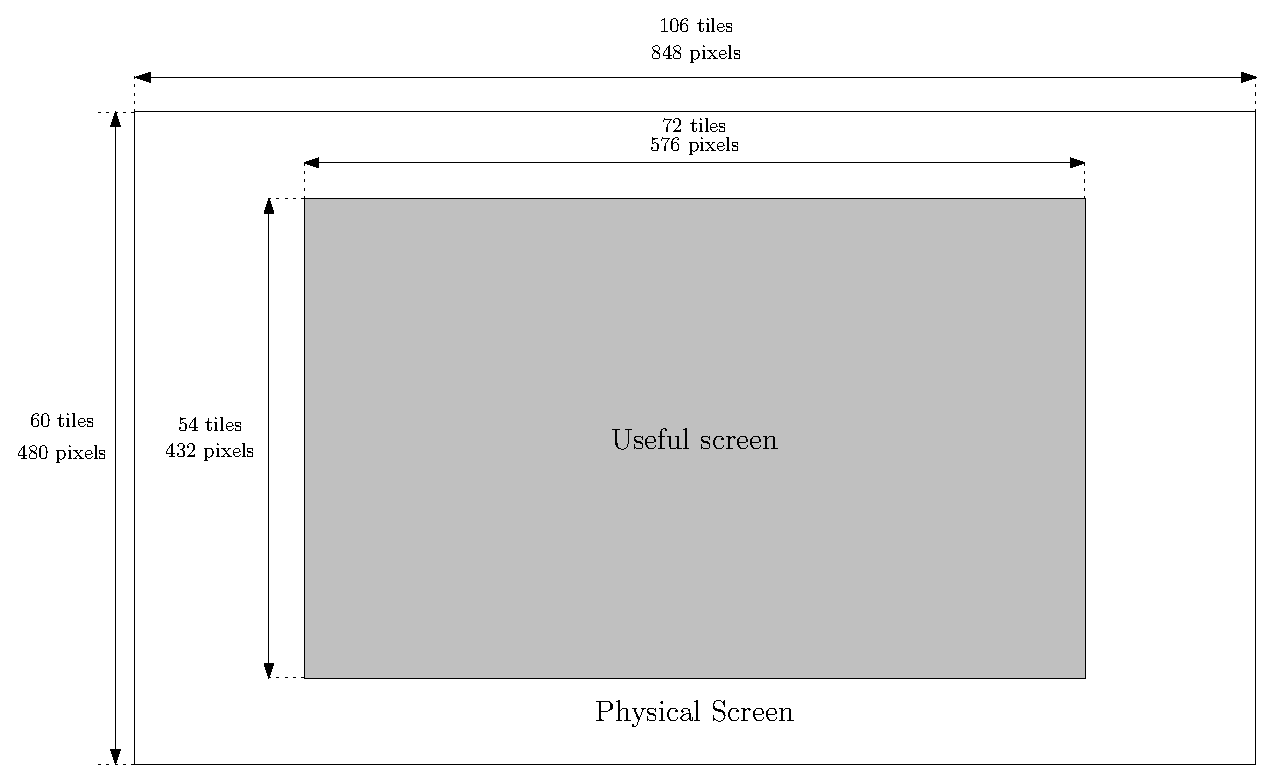
\includegraphics[width=\linewidth]{Chapter4-GPU_CLKU/res/screen_size}
    \caption{Useful screen area in the physical screen}
    \label{fig:gpu/screen_size}
\end{figure}

The problem with putting all tiles in a single memory like this is that only one tile is accessible 
at a time. This means that a mask can only be applied to one tile. This is a pity because it 
prevents the mask from being drawn anywhere on the screen. Indeed, the mask cannot for example be 
drawn between two tiles as shown in Figure \ref{fig:gpu/mask_2tiles}.

\begin{figure}[H]
    \centering
    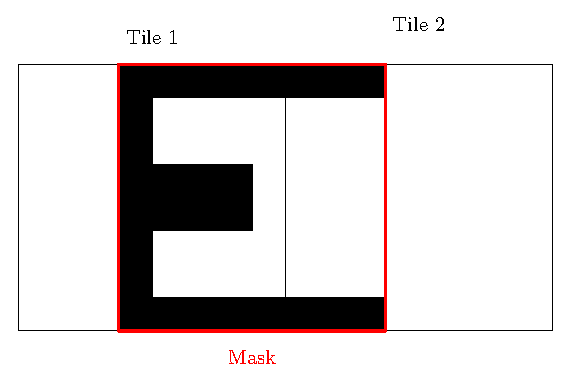
\includegraphics[scale=1.0]{Chapter4-GPU_CLKU/res/mask_2tiles}
    \caption{Mask overlapping two tiles}
    \label{fig:gpu/mask_2tiles}
\end{figure}

When such a placement of the mask takes place, what actually happens is a tile is chosen first. And 
then an offset in pixels is added to the mask. In the example in Figure \ref{fig:gpu/mask_2tiles}, 
the mask has a positive 
offset of N pixels with respect to Tile 1. The idea is then to allow a mask to have an abscissa and
an ordinate offset ranging from 0 to 7. It is not useful to go further than 7 
as this corresponds to placing the mask at the next tile. To be able to apply the mask, it is 
therefore necessary to be able to load four tiles. The first one being the one chosen to draw the 
mask in (x, y), the others being those in (x + 1, y), (x, y + 1) and (x + 1, y + 1). A naive 
solution to load these four tiles would be to have a memory for each tile. However, this has two 
problems. The first one is that this is impossible for the Cyclone V. Indeed, it was seen earlier that 
the Cyclone V has just over 500 M10K memory blocks. However, to represent all the tiles, one would 
need 3888 memories because the definition of a memory in the code must use at least one whole M10K, 
which is simply impossible. Secondly, this would generate way to many connections in the circuits
and a complex multiplexing stage in the memory circuits. This is not tractable for the Cylone V 
neither.

Another way is to try to divide the set of tiles into four groups. These four groups should be 
distributed on the screen in such a way that the placement of a mask loads 4 tiles of different 
groups each time. If one thinks about it, it is possible to convince itself that a simple paving 
of 4 colors allows this (a color represents a group). Figure \ref{fig:gpu/screen_tiling} shows such 
a tiling. 

\begin{figure}[H]
    \centering
    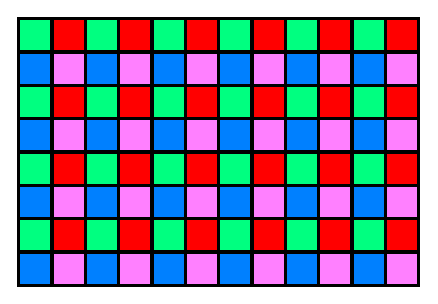
\includegraphics[scale=1.0]{Chapter4-GPU_CLKU/res/screen_tiling}
    \caption{Screen tiling}
    \label{fig:gpu/screen_tiling}
\end{figure}

And the different cases possible by choosing four tiles in the way explained earlier, i.e. one 
tile, the one to the right of it, the one below it and the one at the bottom right are shown in
Figure \ref{fig:gpu/screen_tiling_cases}. It can be seen that in each case, a group is present only 
once, which validates the possibility of representing all tiles using four distinct memories.

\begin{figure}[H]
    \centering
    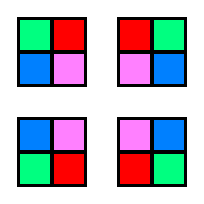
\includegraphics[scale=1.0]{Chapter4-GPU_CLKU/res/screen_tiling_cases}
    \caption{Screen tiling selection cases}
    \label{fig:gpu/screen_tiling_cases}
\end{figure}

\subsection{Mask representation}

A mask has the same dimensions as a tile but does not have the same content. Indeed, a mask can 
contain four different values. The first value is \textit{keep}, corresponding to a 0 in the mask. This 
value means that no modification is made to the pixel targeted by this position in the 
mask. Then there is \textit{set primary}, corresponding to 1, which sets the pixel at this 
location to the primary color, this is better explained later. When the value is 2, 
for \textit{set secondary}, it is then the secondary color that is applied. And 
finally, for the value 3 corresponding to a \textit{reset}, the pixel becomes black. Each of these 
values can therefore be represented on 2 bits. Table \ref{tab:mask_op} summarizes the possible 
operations of a mask.
% PF In general here, I do not see well the constraints imposed by the material vs the design choices.
% PF I am a bit confused: I do not understand the relation to the 4 bits per color in the graphic memory and the primary/secondary color in masks
% PF This is made clear later...


\begin{table}[H]
    \centering
    \begin{tabular}{|l|c|}
    \hline
    \rowcolor[HTML]{DAE8FC} 
    \multicolumn{1}{|c|}{\cellcolor[HTML]{DAE8FC}\textbf{Mask Operation}} & \textbf{Mask Value} \\ \hline
    Keep                                                                  & 0b00                \\ \hline
    Set primary                                                           & 0b01                \\ \hline
    Set secondary                                                         & 0b10                \\ \hline
    Reset                                                                 & 0b11                \\ \hline
    \end{tabular}
    \caption{Mask operations}
    \label{tab:mask_op}
\end{table}

In terms of representation, a mask is a simple vector of 8x8x2 (128) bits. Its LSB corresponds to 
the upper left corner of the mask and its MSB corresponds to the lower right corner of the mask. 
This correspondence is shown in Figure \ref{fig:gpu/mask_vector}.

\begin{figure}[H]
    \centering
    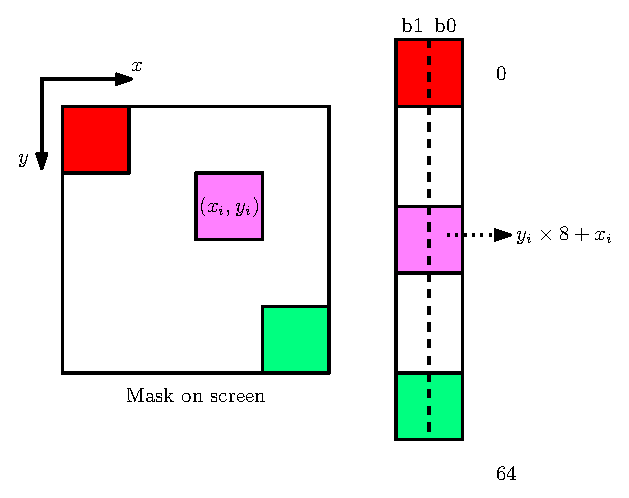
\includegraphics[scale=1.0]{Chapter4-GPU_CLKU/res/mask_vector}
    \caption{Mask vector representation}
    \label{fig:gpu/mask_vector}
\end{figure}

\subsection{Using the GPU}

As introduced, to use the GPU, it is necessary to use the store instruction from the CPU. But the 
address and data must be correctly formatted. For the address, it must start with 0b10 as seen in 
the chapter on the CPU (so that the addressed unit is the GPU). Then, it was decided to make the 
address natural, that is to say that it is 
readable without any conversion. The address therefore contains the exact pixel position where 
a mask should be applied. A pixel being located by four variables: block\_x, block\_y (corresponding 
to the tile), off\_x and off\_y (corresponding to the offset from the tile), these four variables 
are directly present in the address. The format of the address is detailed in 
Figure \ref{fig:gpu/store_address}.

\begin{figure}[H]
    \centering
    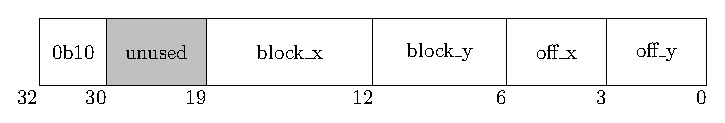
\includegraphics[scale=1.0]{Chapter4-GPU_CLKU/res/store_address}
    \caption{Store instruction address}
    \label{fig:gpu/store_address}
\end{figure}

Concerning the data writen by the store instruction, it must contain the mask identifier and the 
values of the two colors. As a color is 
represented on 12 bits and a word on the CPU is represented on 32 bits, 8 bits remain for the mask.  
The GPU can therefore support 256 masks. The data format is detailed in 
Figure \ref{fig:gpu/store_data}.

\begin{figure}[H]
    \centering
    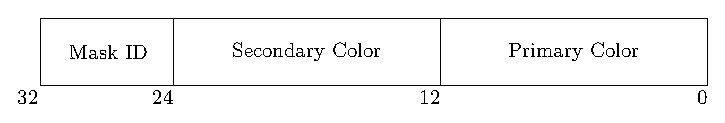
\includegraphics[scale=1.0]{Chapter4-GPU_CLKU/res/store_data}
    \caption{Store instruction data}
    \label{fig:gpu/store_data}
\end{figure}

\subsection{VESA protocol}

The VESA protocol works exactly like the VGA protocol. That is, four signals are present. On the 
one hand there is the 24 bit color signal (8 bits for each primary color, only 4 are truly used
here, the least significant bits are replaced by zeros), the vertical and 
horizontal synchronization signals and the display enable signal. The synchronization signals 
inform the screen of the end of a line for horizontal synchronization and the end of a frame (all 
the lines on a screen) for vertical synchronization. Between two horizontal synchronization 
signals, several things happen. First, there is a pause just after the signal. This time is called 
horizontal back porch. Then, after this pause the colors are sent, the value must be maintained for 
a certain time to fix a pixel. All the pixels of the line are assigned one after the other, in a 
burst. Of course there are specific timing criteria that must be met for this to work, this is 
discussed next. After sending all the colors, a new pause takes place, called horizontal front 
porch. And finally, after this pause, a new horizontal synchronization signal is sent. For the 
frames, it is similar. Before the frame, there is a pause (vertical front porch) followed by the 
vertical synchronization followed by the vertical back porch. Note that the horizontal and vertical 
synchronizations are independent, so both must be evaluated at each moment. When no pause or 
synchronization occurs, either horizontal or vertical, the display is said to be enable. The 
display enable signal is then high and the colors are actually used for the pixels. Outside this 
condition, the color signal can be set to any value and is not listened to. 

The operation of the protocol is shown in Figure \ref{fig:gpu/screen_vesa}. The legend and length
of the signals are available in Table \ref{tab:gpu/vesa}. In this figure, 
the protocol is described in relation to the pixels, and therefore the position on the screen. As 
the screen only includes the pixels of the region where display enable is high, the frame shown is 
a virtual screen, not the physical one, which is smaller. The description is made in relation to the 
pixels because 
it is easier to understand but also to implement. Indeed, as shown later in this report, pixel 
counters are sufficient to implement this protocol. Then, it is enough to fix the right clock 
frequency so that the timings of each pixel are respected. For VESA 848x480, a  33.750MHz clock
is used. Figure \ref{fig:gpu/vesa_signals} shows the value of the signals according to the position
on the screen.

\begin{figure}[H]
    \centering
    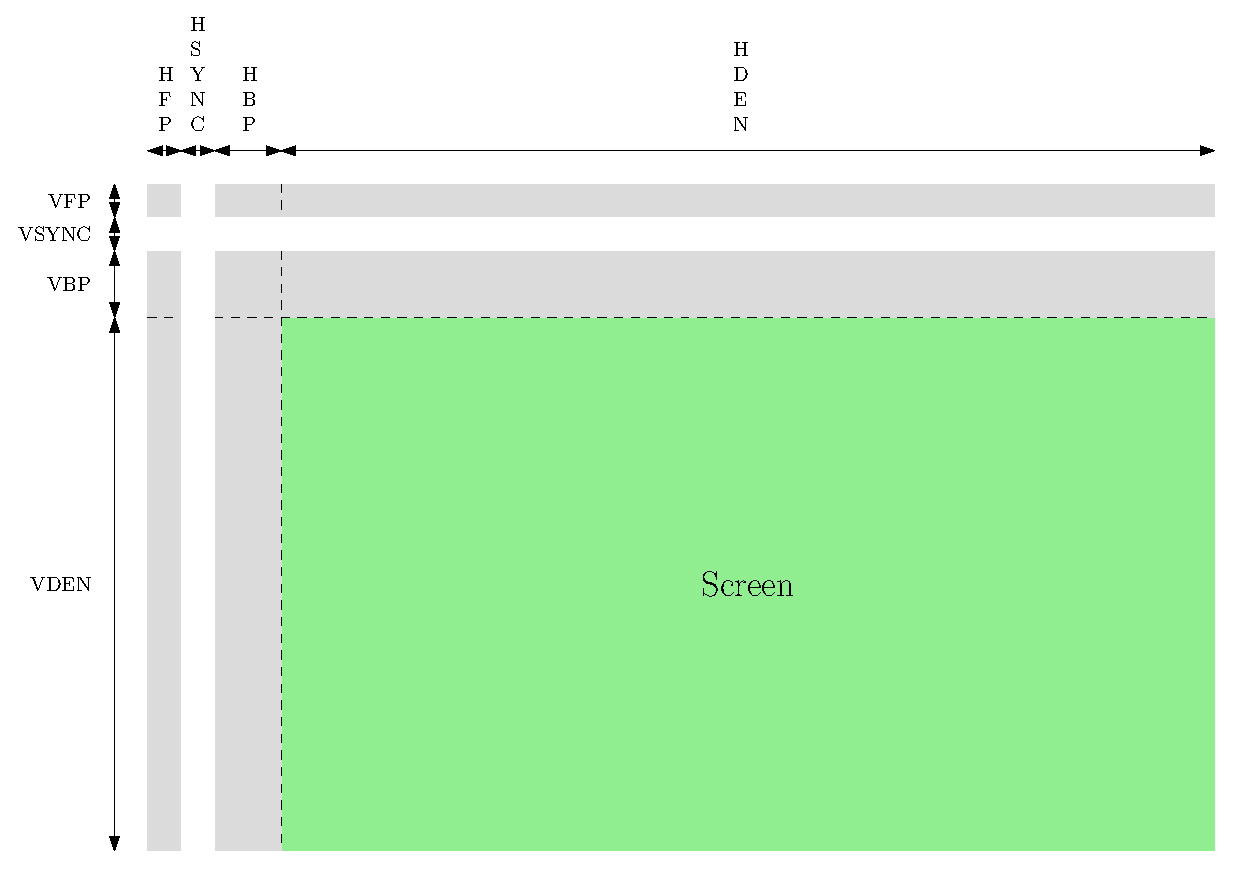
\includegraphics[width=\linewidth]{Chapter4-GPU_CLKU/res/screen_vesa}
    \caption{VESA virtual screen schematic}
    \label{fig:gpu/screen_vesa}
\end{figure}

\begin{table}[H]
    \centering
    \begin{tabular}{|c|c|c|}
    \hline
    \rowcolor[HTML]{DAE8FC} 
    \textbf{Signal} & \textbf{Complete name}    & \multicolumn{1}{l|}{\cellcolor[HTML]{DAE8FC}\textbf{Length (pixels)}} \\ \hline
    HFP             & Horizontal Front Porch    & 16                                                                    \\ \hline
    HSYNC           & Horizontal Sync           & 112                                                                   \\ \hline
    HBP             & Horizontal Back Porch     & 112                                                                   \\ \hline
    HDEN            & Horizontal Display Enable & 848                                                                   \\ \hline
    VFP             & Vertical Front Porch      & 6                                                                     \\ \hline
    VSYNC           & Vertical Sync             & 8                                                                     \\ \hline
    VBP             & Vertical Back Porch       & 23                                                                    \\ \hline
    VDEN            & Vertical Display Enable   & 480                                                                   \\ \hline
    \end{tabular}
    \caption{VESA 848x480 counts}
    \label{tab:gpu/vesa}
\end{table}

\begin{figure}[H]
    \centering
    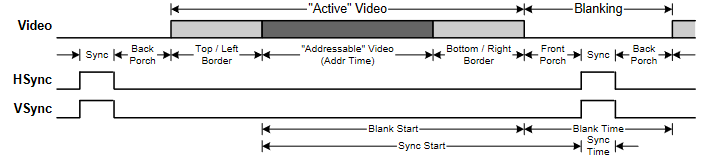
\includegraphics[width=\linewidth]{Chapter4-GPU_CLKU/res/vesa_signals.PNG}
    \caption{VESA signals - video signal represents both display enable signals}
    \label{fig:gpu/vesa_signals}
\end{figure}

\section{GPU components}

\subsection{Graphic memory}

The graphic memory has two functions. The first one is of course to store the state of all the 
pixels of the screen. This is done as discussed above by splitting the memory into four parts. One 
for each group of the Figure \ref{fig:gpu/screen_tiling} tiling. Each of these sub-memories is then 
divided into three memories, one for 
each primary color. This was done this way because it is more optimal to have three memories whose 
word size is a power of two. By dividing by three, each word has 4 bits while it would have had 
12 bits in the case of full colors, which is not a power of 2. A fifth port with a different clock 
from the first 4 ports is also exposed by the graphic memory. This one allows the reading of the 
memory tile by tile for the HDMI controller part of the GPU. This operation is completely independent
of the CPU accesses of this memory, that is why another port is used. The tile loaded from this port
is referred to as Tile b.

The second function is to correctly direct the values in memory to the outputs when reading, and 
the values in input to the memories when writing. Indeed, depending on the editing position (address), the 
current tile belongs to one of the memories. And the memories of the other three tiles to be 
selected also depends on this position. See Figure \ref{fig:gpu/screen_tiling_cases} for the different 
possible configurations. 

From now on, the current tile (at the target position) will be tile 0. The one to the right of it
will be tile 1, the one below it will be tile 2 and the one below it on the right will be tile 3. 
Figure \ref{fig:gpu/tile_ids} summarizes this. Note that the colors are set by tiles. A memory word 
is therefore $4 \times 64$ = 256 bits.

\begin{figure}[H]
    \centering
    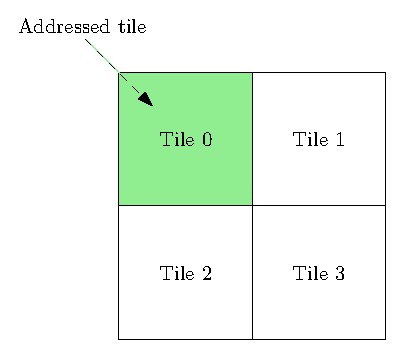
\includegraphics[scale=1.0]{Chapter4-GPU_CLKU/res/tile_ids}
    \caption{Tile identifiers}
    \label{fig:gpu/tile_ids}
\end{figure}

\subsubsection*{Memory unit}

The memory units are the modules representing the groups of tiles, so there are 4 of them in the 
graphic memory. Each memory unit is composed of three Altsyncram configured in true-dualport RAM 
representing the three primary colors. True dualport means that they come with two completely 
independent ports whose clocks are different. The module simply interfaces these three Altsyncrams. 
The internal circuit is given in Figure \ref{fig:gpu/memory_unit_in} and its interface in Figure 
\ref{fig:gpu/memory_unit}. As can be seen, the wren\_b and data\_b signals 
of each memory are grounded since the second port is read-only, that is the one corresponding to
Tile b. The HDMI controller doesn't need to write in memory. For the rest, the signals are 
simply retransmitted. The addresses in the three internal memories are the same since it is the
same tile that is targeted each time. The words are all 256 bits long as each word contains 64 
pixels and one of their color components on 4 bits. 

Now that the memory units are described, it is possible to establish the complete memory circuit.
The complete circuit is shown in Figure \ref{fig:gpu/memory_in}. It consists of a parallel 
connection of four memory units. 

Each color input of each memory unit is multiplexed between the four color inputs of the same color. 
The four inputs of these multiplexers are in fact the colors of each of the 
tiles used (tile 0, tile 1, tile 2 and tile 3). Then, each of the outputs of the memory are 
multiplexed from the values in memory in the different memory units. All these multiplexers ensure 
that the tiles are correctly routed, as explained above. These multiplexers are controlled by five 
signals: sw0, sw1, sw2, sw3 and swb which are respectively linked to tile 0, tile 1, tile 2, tile 3 
and tile b. The determination of the values of these switches as well as those of the addresses of 
the memory units are not displayed in the circuit for simplicity. But their
value are simply based on the selected tile location, Tile 0. Depending on its location, it belongs 
to one of the four tile groups. The groups of the neighbor tiles are also computed based on the 
locations of these tiles and their respective switches are set according to the group of the tile. 

\begin{figure}[H]
    \centering
    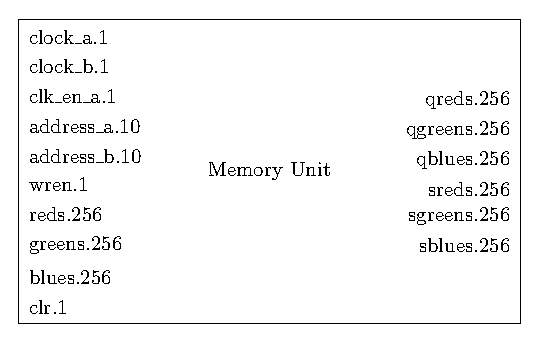
\includegraphics[scale=1.0]{Chapter4-GPU_CLKU/res/memory_unit}
    \caption{Memory Unit}
    \label{fig:gpu/memory_unit}
\end{figure}

\begin{figure}[H]
    \centering
    
\includegraphics[scale=1.0]{Chapter4-GPU_CLKU/res/memory_unit_in}
    \caption{Memory Unit internal circuit}
    \label{fig:gpu/memory_unit_in}
\end{figure}

\begin{figure}[H]
    \centering
    
\includegraphics[scale=0.55]{Chapter4-GPU_CLKU/res/memory_in_part1}
    \caption{Memory internal circuit}
    \label{fig:gpu/memory_in}
\end{figure}

The interface of the memory can be found in Figure \ref{fig:gpu/memory}. 
The red, green and blue signals of each tile 
are put together in a bus to simplify the representation of the module.

\begin{figure}[H]
    \centering
    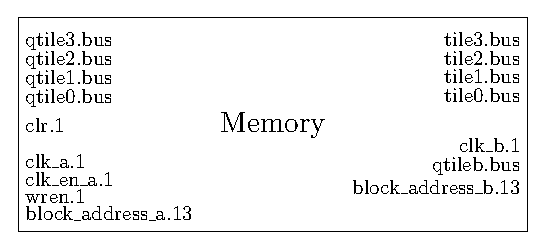
\includegraphics[scale=1.0]{Chapter4-GPU_CLKU/res/memory}
    \caption{Memory}
    \label{fig:gpu/memory}
\end{figure}

\subsection{Mask memory}

The mask memory is identical to the CPU instruction memory except that the Altsyncram used contains 
only 256 words of 128 bits. This allows to store 256 masks. The circuit is given in Figure
\ref{fig:gpu/mask_memory_in} and \ref{fig:gpu/mask_memory} provides its interface. Note that if the 
address is equal to 255, then the mask sent to the data\_read output is a constant mask 
(named clear mask) which clears all pixels.

\begin{figure}[H]
    \centering
    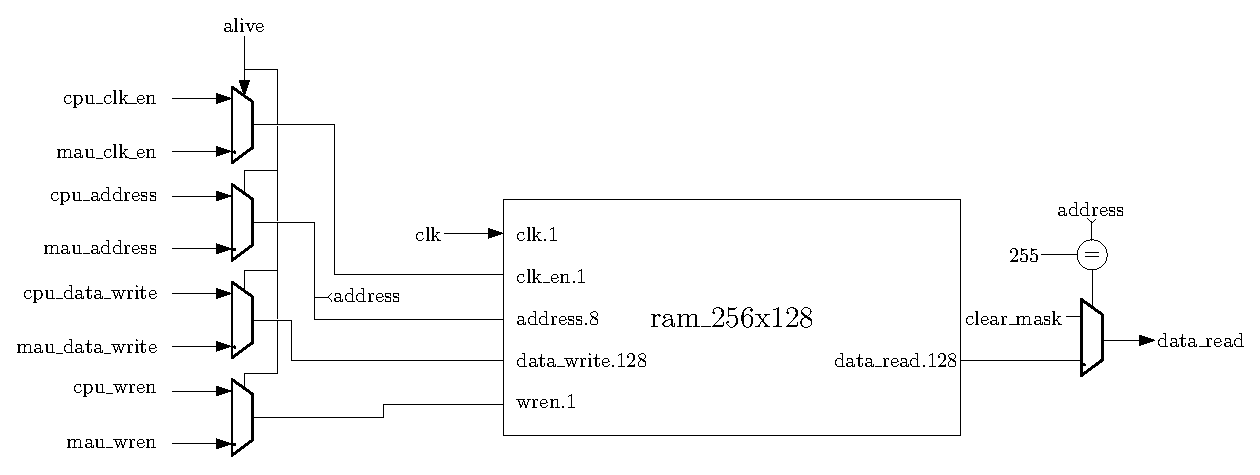
\includegraphics[width=\linewidth]{Chapter4-GPU_CLKU/res/mask_memory_in}
    \caption{Mask memory internal circuit}
    \label{fig:gpu/mask_memory_in}
\end{figure}

\begin{figure}[H]
    \centering
    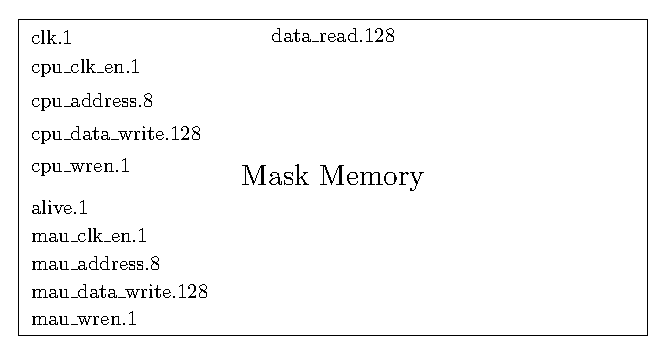
\includegraphics[scale=0.8]{Chapter4-GPU_CLKU/res/mask_memory}
    \caption{Mask memory}
    \label{fig:gpu/mask_memory}
\end{figure}

\subsection{Shifter}

The objective of this module is to replicate the mask four times and to shift it in each of these 
copies so that it corresponds to the mask offset given by the user. After that, each of the copies 
can be associated with one of the four tiles loaded out of memory. This association is done in 
another module.

\subsubsection*{Shifter Unit}

This module is responsible for shifting. To do this it simply takes the signed 
offsets given in input and shifts the bits of the mask. The offsets being given in pixels and the
masks having two bits per pixel, it is necessary to multiply by two each offset. To achieve an 
horizontal offset, each line of the mask is shifted 2 $\times$ offset\_x while for a vertical offset, the whole mask is shifted of 16 $\times$ offset\_y given that there are 8 pixels 
by line. The circuit and the interface of the shifter unit are respectively given in Figures
\ref{fig:gpu/shifter_unit_in} and \ref{fig:gpu/shifter_unit}.

\begin{figure}[H]
    \centering
    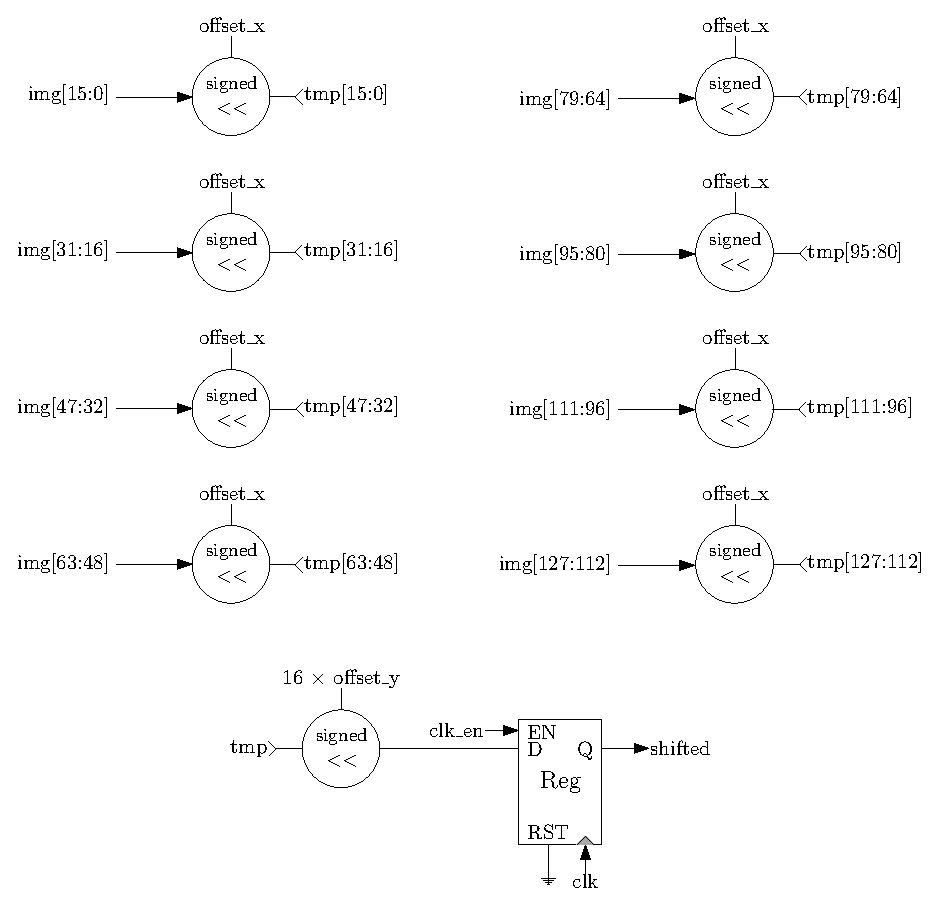
\includegraphics[width=\linewidth]{Chapter4-GPU_CLKU/res/shifter_unit_in}
    \caption{Shifter unit internal circuit}
    \label{fig:gpu/shifter_unit_in}
\end{figure}

\begin{figure}[H]
    \centering
    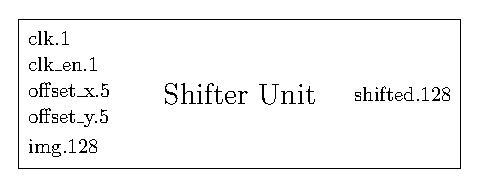
\includegraphics[scale=0.8]{Chapter4-GPU_CLKU/res/shifter_unit}
    \caption{Shifter unit}
    \label{fig:gpu/shifter_unit}
\end{figure}

The complete shifter is just a simple parallelization of four shifters but one has to choose the right 
offsets for each shifter unit. In Figure \ref{fig:gpu/shifter_offsets} are shown
the different offsets needed to obtain the desired masks. Each offset is taken with respect to the 
upper left corner of the mask to which it is associated. off\_0 is of course equal to 
(off\_x, off\_y) since the offset is always given from the selected tile and the selected tile is 
identified by id 0. For the others, the offsets are off\_1 = (off\_x - 8, off\_y), off\_2 = 
(off\_x, off\_y - 8) and off\_3 = (off\_x - 8, off\_y - 8).

\begin{figure}[H]
    \centering
    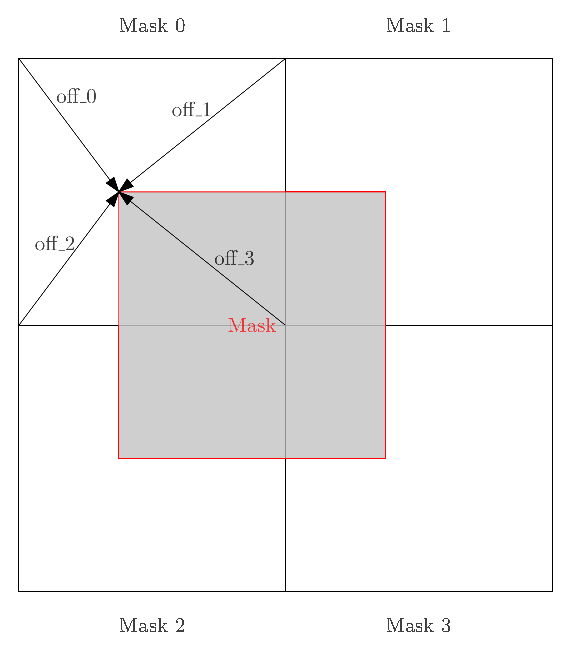
\includegraphics[scale=1.0]{Chapter4-GPU_CLKU/res/shifter_offsets}
    \caption{Masks offsets}
    \label{fig:gpu/shifter_offsets}
\end{figure}

The complete shifter circuit can then be established and is given in Figure \ref{fig:gpu/shifter_in}. 
Figure \ref{fig:gpu/shifter} contains the shifter interface.

\begin{figure}[H]
    \centering
    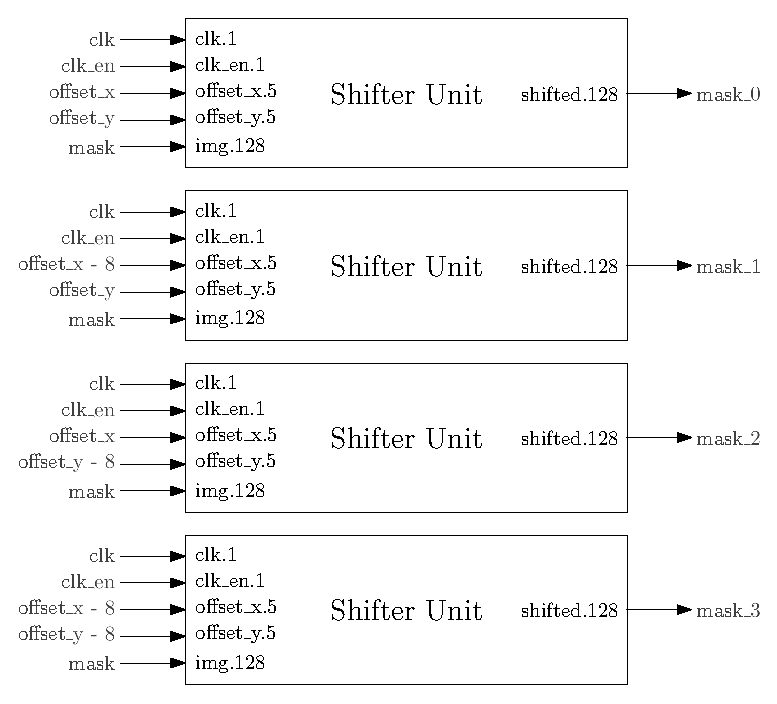
\includegraphics[scale=1.0]{Chapter4-GPU_CLKU/res/shifter_in}
    \caption{Shifter internal circuit}
    \label{fig:gpu/shifter_in}
\end{figure}

\begin{figure}[H]
    \centering
    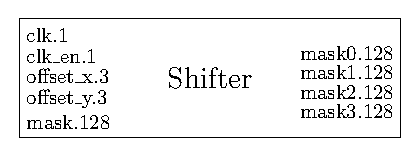
\includegraphics[scale=1.0]{Chapter4-GPU_CLKU/res/shifter}
    \caption{Shifter}
    \label{fig:gpu/shifter}
\end{figure}


\subsection{Mask Logic Unit (MLU)}

The MLU is simply used to modify the current value of a pixel in a tile according to the operation 
described for this pixel in the corresponding mask. This module is a kind of giant multiplexer. In 
fact, it contains a multiplexer for each primary color of each pixel and will select an input 
(the current value of the pixel, the primary color, the secondary color or the black color) 
according to the value of the mask at that position. Its operation is very simple to understand 
and its circuit impossible to draw on a page of this report, so the circuit is not detailed here. The interface is however given in Figure \ref{fig:gpu/mlu}.
Note that this circuit is completely combinatorial. Concerning the tile buses, they are simply
made up of the three color signals of the corresponding tile.

\begin{figure}[H]
    \centering
    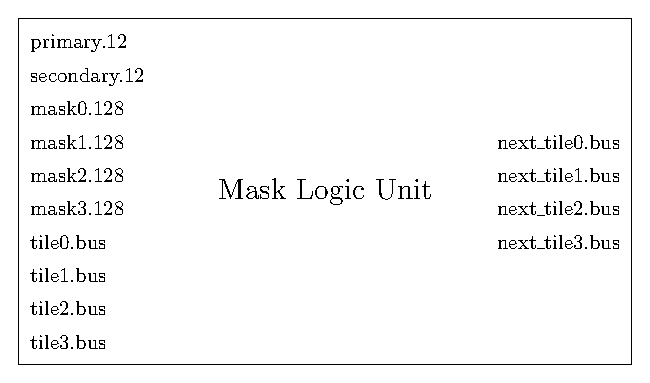
\includegraphics[scale=1.0]{Chapter4-GPU_CLKU/res/mlu}
    \caption{Mask Logic Unit}
    \label{fig:gpu/mlu}
\end{figure}

\subsection{Graphic Counter (GC)}

The graphics counter is the first element fully included in the HDMI controller part of the GPU. 
It simply counts and provides several counts. First, it provides the current position of the 
pixel taken into account, so cnt\_h and cnt\_v representing the horizontal and vertical position 
of the pixel. These go through all the virtual screen of the VESA, that is to say from 0 to 1087 
for cnt\_h and from 0 to 516 for cnt\_v. These counts are then used to correctly generate the 
synchronization signals of the VESA in another module. 

Then, it provides four other counters blk\_x, blk\_y, off\_x, off\_y which again give the position 
of a pixel but using this time the GPU coordinate system. It should be noted that these counters 
only count from the start of the useful screen. In other words, blk\_x and blk\_y are both at 0 
when cnt\_h and cnt\_v correspond to the location of the first pixel of the first tile in 
memory, the one at the top left corner of the useful screen. And their values continue to increase 
until the end of the VESA virtual screen.

Notice also that the useful screen does not correspond to the entire active area of the 
VESA. As mentioned earlier, not all the space is used because of memory constraints. The useful 
screen is centered in this active region. When the counter is in the useful region of the screen, 
the in\_mem signal is high to warn that the position given by the counter corresponds to a tile 
present in memory. The range of the counters and a schematic of the positioning of the useful 
region are given in Figure \ref{fig:gpu/gc_screen}.

\begin{figure}[H]
    \centering
    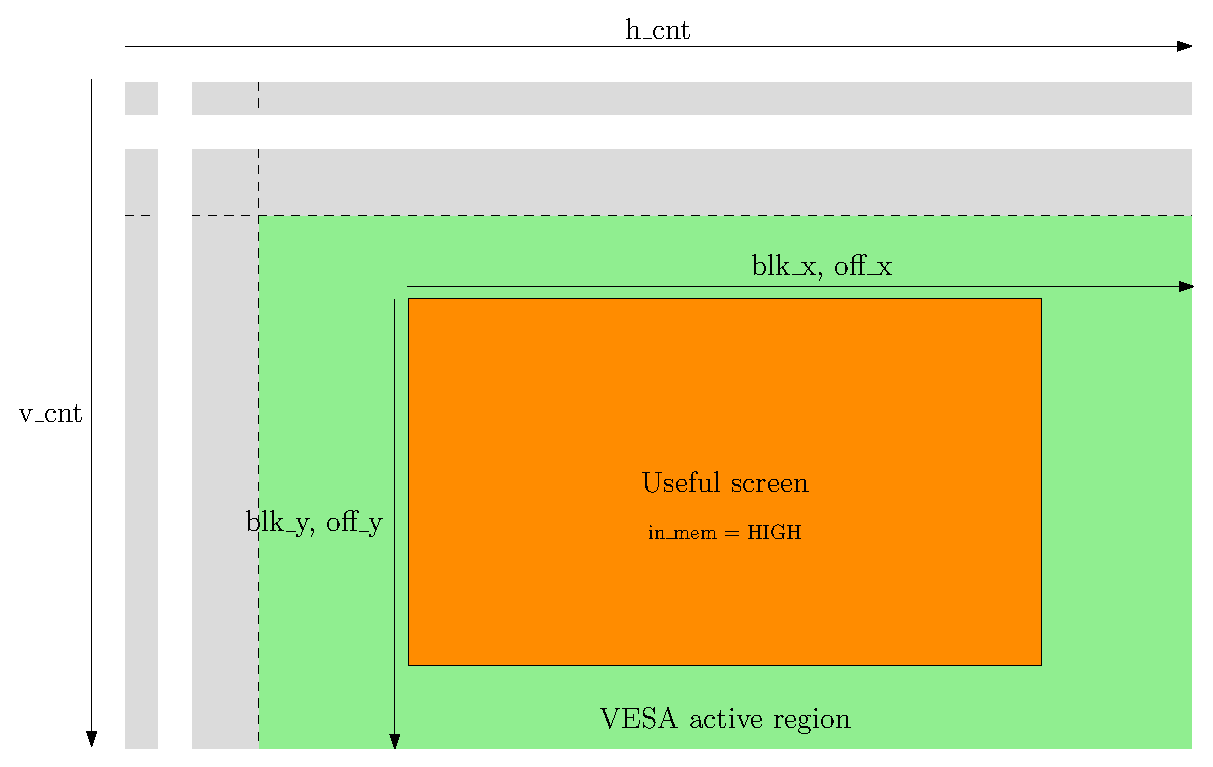
\includegraphics[width=\linewidth]{Chapter4-GPU_CLKU/res/gc_screen}
    \caption{Counters range and useful screen}
    \label{fig:gpu/gc_screen}
\end{figure}

All these counters are implemented with the help of registers by choosing correctly the clk\_enable 
signals and the reset signals. The inner circuit without the in\_memory which is only a condition 
on the values of h\_cnt and v\_cnt is given in Figure \ref{fig:gpu/gc_in}. The interface is also shown in Figure \ref{fig:gpu/gc}.

\begin{figure}[H]
    \centering
    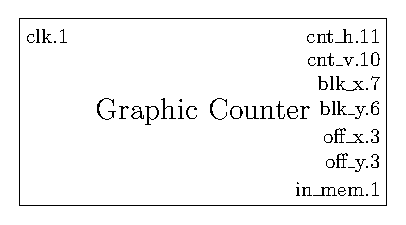
\includegraphics[scale=0.8]{Chapter4-GPU_CLKU/res/gc}
    \caption{Graphic counter}
    \label{fig:gpu/gc}
\end{figure}

\begin{figure}[H]
    \centering
    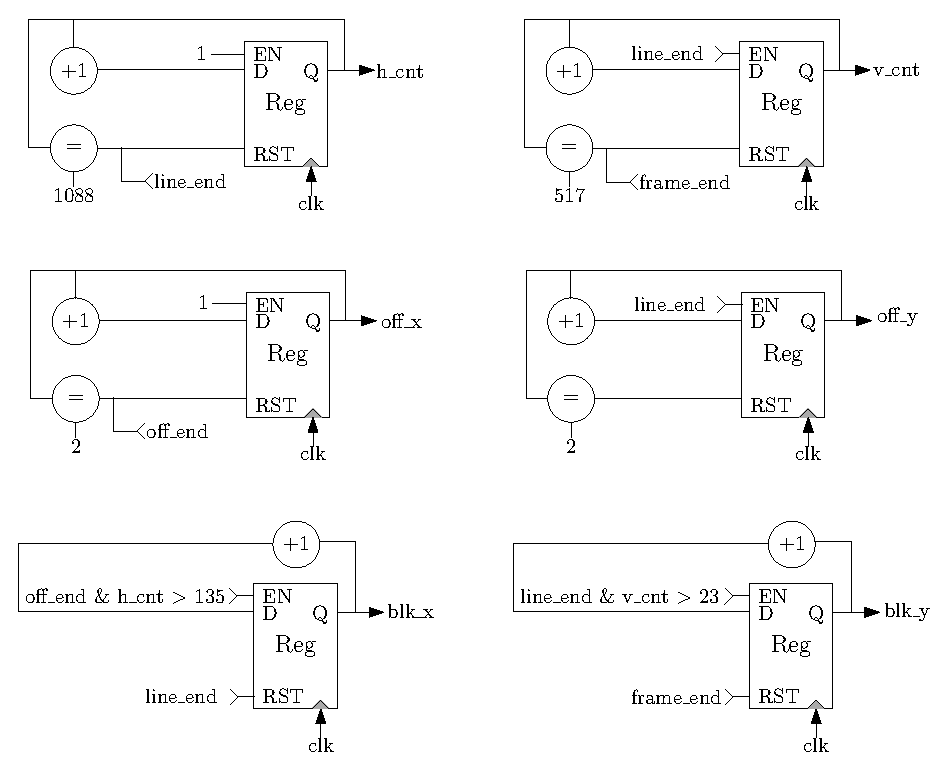
\includegraphics[width=\linewidth]{Chapter4-GPU_CLKU/res/gc_in}
    \caption{Graphic counter internal circuit}
    \label{fig:gpu/gc_in}
\end{figure}

\subsection{Synchronizer}

The synchronizer is in charge of generating the synchronization and display enable signals of the
VESA protocol. It simply looks at the values of the h\_cnt and v\_cnt signals provided by the 
graphic counter. If the values are within the ranges associated with the synchronizations or display
enable, the synchronizer sets the signal to high. As a reminder, the ranges were described in 
Figure \ref{fig:gpu/screen_vesa} and Table \ref{tab:gpu/vesa}. As the internal circuit is 
only a condition, it is not shown. The interface is shown in Figure \ref{fig:gpu/synchronizer}.  

\begin{figure}[H]
    \centering
    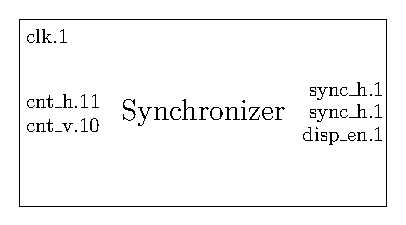
\includegraphics[scale=1.0]{Chapter4-GPU_CLKU/res/synchronizer}
    \caption{Synchronizer}
    \label{fig:gpu/synchronizer}
\end{figure}

\subsection{I2C HDMI Config}

This module is provided by Terasic to configure the HDMI controller present on the DE10 nano board. 
In this work, it is used as a library, i.e., its description is not detailed here since it has been used as a black box. In the GPU, it is simply connected to the pins of the physical
HDMI controller as Terasic suggests in its tutorial. The interface is provided in 
Figure \ref{fig:gpu/i2c}.

\begin{figure}[H]
    \centering
    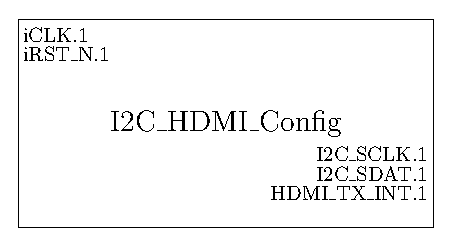
\includegraphics[scale=0.8]{Chapter4-GPU_CLKU/res/i2c}
    \caption{I2C HDMI Config}
    \label{fig:gpu/i2c}
\end{figure}

\subsection{Complete circuit}

The GPU whose internal circuit is given in Figure \ref{fig:gpu/gpu_in}, like the CPU, runs in 
sequence. It starts by reading the mask in the mask memory. Then it reads the tiles to be edited in 
the memory and shifts the masks at the same time. The results of these two operations arrive in the 
mask logic unit where they are processed in a combinatorial way. Each mask operates on the tile 
associated to it, taking into account the primary and secondary colors. Once this is done, the 
memory is enabled again, in writing mode this time. 

Similarly to some CPU memories, the mask memory has a MAU access that allows reading and writing of this 
memory from the ARM processor.

This constitutes the computational part of the GPU, the one that the CPU controls through its ST and 
LD operations. 

Then, there is the controller that fetches each tile in memory one by one and draws all the pixels
on the physical screen. 
It also manages the synchronization signals of the VESA protocol. The graphic counter is used to 
provide the address of the memory. To do this, the blk\_x and blk\_y outputs are concatenated to 
form the address. Then, the offsets are added together to form an index in the tile and select the current 
pixel. The selected pixel is then put on the output if the signal in\_memory of the graphic counter 
is high, otherwise the color is black. It is to this effect that the two multiplexers are used on 
the hdmi\_tx\_d output. It should be noted that the index and the im\_mem signal must be delayed so 
that they arrive at the multiplexers at the same time as the tile requested from the memory. This 
is why two registers are left on their way. The cnt\_h and cnt\_v signals go to the synchronizer 
which is responsible for generating the synchronization signals. And finally, there is also the 
I2C\_HDMI\_Config to configure the physical HDMI controller.

It should be noted that two clocks are present. On the computational side, it is the same clock as 
the CPU that is used to ensure that the two modules are synchronized. On the HDMI side, it is the 
VESA protocol clock that is used. It is called gpu\_clk. The GPU interface is available in Figure
\ref{fig:gpu/gpu}.

\begin{figure}[H]
    \centering
    
\includegraphics[width=\linewidth]{Chapter4-GPU_CLKU/res/gpu_in}
    \caption{GPU internal circuit}
    \label{fig:gpu/gpu_in}
\end{figure}

\begin{figure}[H]
    \centering
    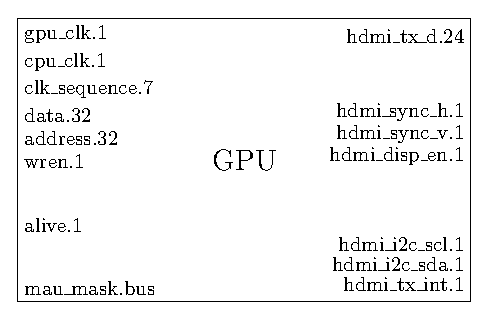
\includegraphics[scale=1.0]{Chapter4-GPU_CLKU/res/gpu}
    \caption{GPU}
    \label{fig:gpu/gpu}
\end{figure}

\section{Clock Unit (CLKU)}

As seen previously, two clocks are needed. One as high as possible for the CPU and the modules 
working synchronously with it and one for the 33.750MHz HDMI controller. The CPU clock cannot 
exceed 50MHz. Indeed, other higher frequencies have been tested but do not meet the timing 
constraints at compile time. For the CPU, the clock unit only passes the FPGA 50MHz physical clock 
from the input to the output (the CPU clock circuit is a simple wire). For the GPU clock, the frequency
has to be modified. This is done 
using a PLL (Phased-locked loop) which allows to generate a clock with a given frequency from 
another clock with a fixed frequency. This PLL is easily configured in a GUI using the Quartus 
Mega Wizard by setting the input and output frequencies. The CLKU then consists in a PLL. Its interface 
is given in Figure \ref{fig:clku/clku}.

\begin{figure}[H]
    \centering
    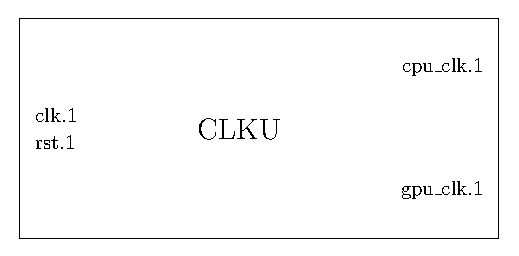
\includegraphics[scale=1.0]{Chapter4-GPU_CLKU/res/clku}
    \caption{CLKU}
    \label{fig:clku/clku}
\end{figure}

\chapter{Memory Access Unit and Control Unit design}

In this section the Memory Access Unit is described, which gives the ARM part read and write 
access to several memories of the system. Another super-unit, the Control Unit is also described here. 
The latter keeps the state of the machine (on or off) and gives access to this register to the 
ARM part. The ARM processor can therefore switch the machine on and off as it wishes from this 
access. Before introducing these two super-units, the Avalon protocol is first described. This 
protocol allows the communications through the bridges existing between the ARM and FPGA part of
the Cyclone V.

\section{Communication between ARM and FPGA sides}

The communication between the two parts takes place via one of the priously mentionned bridges using 
the Avalon protocol described by Intel. This protocol allows 
high-speed communication. The Avalon interface has different sub-interfaces for different types 
of communication. Each type is adapted to certain applications. In this project where the protocol 
is used to communicate between master and slave devices, the Avalon MM is used. 
The Avalon MM protocol is address based which is very suitable for the needs of this project.
The read and write operations of this protocol are described right below.

\subsection{Read operation}

First, let's start by reading. The sequence diagram of the protocol for the reading operation is 
visible in Figure \ref{fig:avalon/mm_read}. In the diagram, two masters are represented but only 
the unique master case is described. In the first place, the master simply has to give
the start address to which it wants to read, the length of the burst (the number of words desired) 
as well as to switch the read and beginbursttransfer signals to high. The slave then responds 
to this with a waitrequest that goes up. The master must imperatively keep all signals except 
beginbursttransfer which returns to the low state unchanged during the waitrequest to give the 
slaves time to capture them. Once ready, the slave removes the waitrequest and informs that  
data is available by switching readdatavalid to high and sending the first word. The other words 
are then sent to the master in the order of their addresses. 

\begin{figure}[ht!]
  \center
  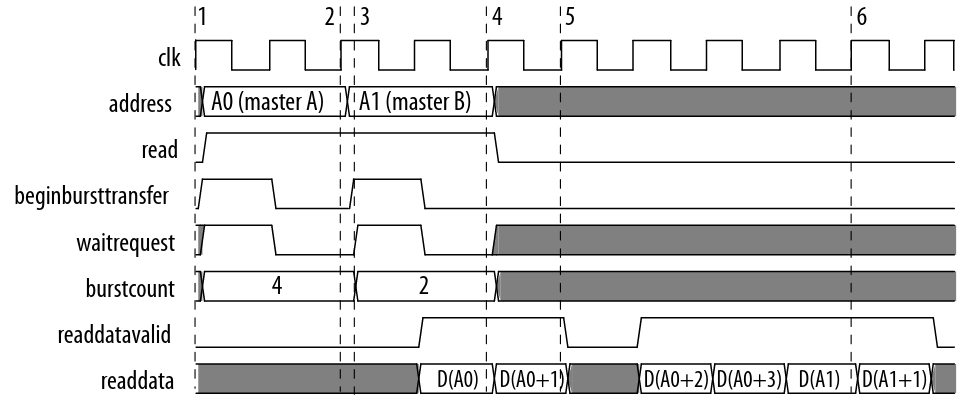
\includegraphics[width=\linewidth]{"Chapter5-MAU_CTRLU/res/avalon_mm_read.png"}
  \caption{Read operation using Avalon MM}
  \label{fig:avalon/mm_read}
\end{figure}

\subsection{Write operation}

For writing, it's even simpler. As can be seen in Figure \ref{fig:avalon/mm_write}, the beginning 
is similar to reading. The master has to provide the first address, the length of the 
burst and also to switch beginbursttransfer to high. In addition to that, the first word 
is also provided. Here again, the slave responds with a waitrequest. As soon as the waitrequest 
is switched off, the master sets the beginbusttransfer to low and send the words one after the other, 
starting at the next clock cycle. If the write signal goes down, the burst is paused and resumes 
as soon as it goes up again.

\begin{figure}[ht!]
  \center
  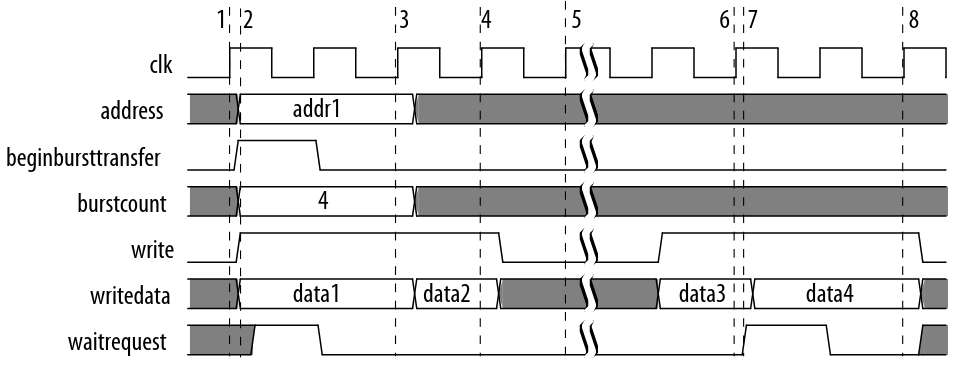
\includegraphics[width=\linewidth]{"Chapter5-MAU_CTRLU/res/avalon_mm_write.png"}
  \caption{Write operation using Avalon MM}
  \label{fig:avalon/mm_write}
\end{figure}

This protocol is not very complicated. However, it has a lot of signals and is not necessarily 
practical to use directly in user-developed slaves and masters. This is why interface modules are 
used. These modules are described in the sections where they are needed.

\section{Memory Access Unit (MAU)}

As already repeated several times the MAU allows access to several memories of the machine. In order 
to simplify the protocol in the machine, a module called Avalon to External Bus Bridge is used. This 
module manages the Avalon protocol and exposes an interface (the external bus) using a simpler 
protocol. This module is used as many times as there are memories to connect to the interconnect.
The different signals this module uses are shown in Figure \ref{fig:mau/bus_bridge}. Note that this
module has an integrated timer that is reset each time the Avalon to external bus bridge receives
an acknowledgement from the external slave. When this timer reaches 0, the request from the master 
(denoted by Avalon Switch Fabric in the Figure) is deleted.

\begin{figure}[ht!]
    \center
    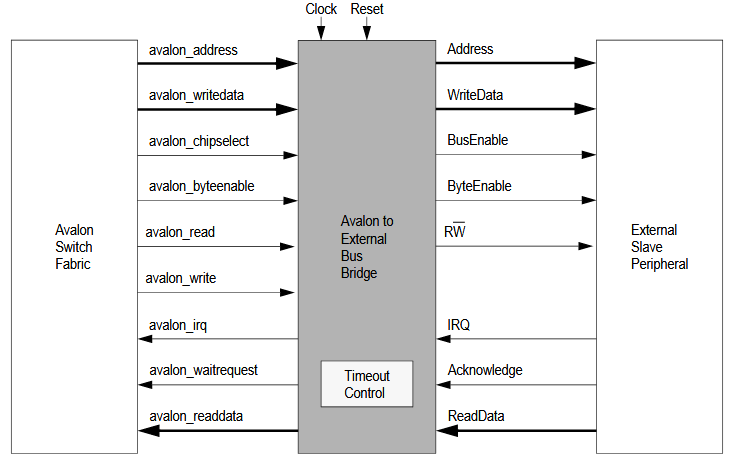
\includegraphics[scale=0.8]{"Chapter5-MAU_CTRLU/res/external_bus_bridge.PNG"}
    \caption{Avalon to external bus bridge interface and signals}
    \label{fig:mau/bus_bridge}
\end{figure}

The protocol is considered simpler because it offers an interface closer to that used by the memories 
than that of the Avalon. Indeed, the usual signals address, write data, read data and R$\overline{W}$ are 
present. Moreover, this protocol is very simple to use. Indeed, as can be seen in Figure \ref{fig:mau/bus_bridge_protocol}. The master 
places all the necessary elements on the bus and then switches the bus enable signal to high. This means 
that the slave can act. The slave then does what it has to do. Either take the data and write it to 
the address given by the master or send the requested data that is present at the address given by 
the master. Once the slave has finished its job, it switches the acknowledgement signal to high 
during a clock cycle to validate the transaction. 

\begin{figure}[ht!]
    \center
    \includegraphics[scale=0.8]{"Chapter5-MAU_CTRLU/res/external_bus_timings.PNG"}
    \caption{External bus protocol timings}
    \label{fig:mau/bus_bridge_protocol}
\end{figure}

It is possible to configure the address range and the word size used by these bus. For this work, 
it is decided that the 
addressable space is 256Kbytes long and that the words are on 32bits for each access except for the 
access to the GPU mask memory which is on 4Kbytes with 128bits words. Each of these accesses are 
put on the HPS-FPGA bridge, their offset is given in Table \ref{mau/bus}. These dimensions were 
chosen to make the offset easy to understand. Indeed, only the sixth number changes in the 
hexadecimal address. Moreover, this gives future users a large margin if they want to change the 
dimensions of the memories. As far as the mask memory is concerned, the address range is simply the 
size of the memory. This has been done especially to discourage any modification at this level. 
Indeed, this would lead to a large modification of the GPU which could degrade its performance or 
make it impossible to include in the design (due to lack of space on the FPGA).

\begin{table}[ht!]
    \centering
    \begin{tabular}{|l|c|c|c|c|}
    \hline
    \rowcolor[HTML]{DAE8FC} 
    \multicolumn{1}{|c|}{\cellcolor[HTML]{DAE8FC}\textbf{Access}} & \textbf{Base} & \textbf{End} & \textbf{Address range} & \textbf{Word size} \\ \hline
    Instruction Memory (CPU)                                      & 0x0000 0000   & 0x0003 FFFF  & 256kB             & 32                 \\ \hline
    Data Memory (CPU)                                             & 0x0010 0000   & 0x0013 FFFF  & 256kB             & 32                 \\ \hline
    Register File (CPU)                                           & 0x0020 0000   & 0x0023 FFFF  & 256kB             & 32                 \\ \hline
    I/Os (IOU)                                                    & 0x0030 0000   & 0x0033 FFFF  & 256kB             & 32                 \\ \hline
    Mask Memory (GPU)                                             & 0x0040 0000   & 0x0040 0FFF  & 4096B             & 128                \\ \hline
    \end{tabular}
    \caption{Memory bus description}
    \label{mau/bus}
\end{table}

The connections in QSys are shown in Figure \ref{fig:avalon/bus}. 
The different modules and the HPS are highlighted in 
yellow. The different Avalon slaves and the master are shown in red. It can be noticed by following 
the connection highlighted in blue that it is indeed the HPS-FPGA bridge that is used 
(h2f\_axi\_master in Qsys) and that the offsets of the slaves are indeed those previously given. The 
signals corresponding to the buses are displayed in green. Each of them is exported, that is to say 
that they can be used from the FPGA. They are the ones that are connected to the different memories.

\begin{figure}[ht!]
    \center
    \includegraphics[width=\linewidth]{"Chapter5-MAU_CTRLU/res/qsys_mau.PNG"}
    \caption{Avalon to external bus bridges connections in Qsys}
    \label{fig:avalon/bus}
\end{figure}

Now that the descriptions of the external bus bridge and its implementation are done, the design of 
the MAU can be considered.

\subsection{Memory Access}

In fact, the Memory Access Unit is composed of only two types of modules. The Memory Access 32, and 
the Memory Access 128 allowing both the interfacing between an external bus and a memory (these two
modules respectively have words of 32 and 128 bits). To do this, they both implement a finite state machine. 
That of Memory Access 32 is given in Figure \ref{fig:ma_fsm}. The only difference that the 128 bits version 
has is that the address is not multiplied by 4 in the Iddle state. 

\begin{figure}[ht!]
    \center
    \includegraphics[scale=0.8]{"Chapter5-MAU_CTRLU/res/mau_fsm"}
    \caption{Memory Access 32 finite state machine}
    \label{fig:ma_fsm}
\end{figure}

This state machine simply follows the protocol described earlier. It only acts when the bus is high 
and sends an acknowledge during a clock cycle once the request is executed (the finite state machine 
is reevaluated at each clock cycle). On the read side, a state seems to be useless (Read 1). This 
one is in fact very important, it gives the memory time to fetch the value present at the requested 
address. The interfaces of the memory acess are given in Figures \ref{fig:ma32} and \ref{fig:ma128}.

\begin{figure}[ht!]
    \center
    \includegraphics[scale=0.8]{"Chapter5-MAU_CTRLU/res/memory_access_32"}
    \caption{Memory Access 32}
    \label{fig:ma32}
\end{figure}

\begin{figure}[ht!]
    \center
    \includegraphics[scale=0.8]{"Chapter5-MAU_CTRLU/res/memory_access_128"}
    \caption{Memory Access 128}
    \label{fig:ma128}
\end{figure}

\subsection{Memory Access Unit circuit}

The Memory Access Unit is therefore a simple parallelization of four Memory Access 32 modules and 
one Memory Access 128 module. The MAU will later be connected to the different signals exported to 
QSys. The circuit of the MAU is given in Figure \ref{fig:mau_in} and its interface is shown in 
Figure \ref{fig:mau}. In order to simplify the interface of the MAU, not all signals are put in it 
and a bus representation is used. However, all signals are available in the internal circuit.

\begin{figure}[ht!]
    \center
    \includegraphics[width=\linewidth]{"Chapter5-MAU_CTRLU/res/mau_in"}
    \caption{Memory Access Unit internal circuit}
    \label{fig:mau_in}
\end{figure}

\begin{figure}[ht!]
    \center
    \includegraphics[scale=0.8]{"Chapter5-MAU_CTRLU/res/mau"}
    \caption{Memory Access Unit}
    \label{fig:mau}
\end{figure}

\section{Control Unit (CTRLU)}

The control unit is a very simple unit. It manages the state of the machine. By managing the state is meant that 
it decides whether the machine is switched on or off. Initially, the machine is switched off (alive 
in the low state). When alive is low, the memories of the machine can be manipulated by the ARM 
processor. It is thus at this moment that the machine is programmed. Once this is done, the ARM 
processor can start the machine by switching alive to the high state, the means by which this is 
achieved are seen just after. During the execution of a program, it can be stopped in two ways. 
Firstly by the ARM processor which can force the stop, by passing alive to the low state. Secondly, 
the beta machine itself can order the stop by executing the EXIT instruction which will change the 
halt signal to high. The control unit will then respond to this signal by switching alive to low.

As for the MAU, it is necessary to connect a module to the interconnect to make this unit 
accessible from the ARM processor. Once again, the Avalon protocol is not used directly. 
Instead, a module called Parallel IO (PIO) is used. This one gives direct access to a register 
from the interconnect (and thus from the ARM processor). This module also uses the MM avalon, so 
the register has an address from the point of view of the ARM processor. A difference with 
the Avalon to external bus bridge of the MAU is that the PIO is put on the lightweight HPS-FPGA 
bridge. This choice is made because the PIO is not frequently used and does not require large data 
transfers. For this kind of modules, the HPS documentation advises to use the lightweight.

The connection of the parallel IO in QSys is shown in Figure \ref{fig:qsys/ctrlu}. The same color 
code as usual is used.

\begin{figure}[ht!]
    \center
    \includegraphics[width=\linewidth]{"Chapter5-MAU_CTRLU/res/qsys_ctrlu.PNG"}
    \caption{Parallel IO connections in QSys}
    \label{fig:qsys/ctrlu}
\end{figure}

One of the ports is exported. In fact this one exposes two signals. One input and one output. The 
output allows to read what the ARM processor proposes as new value of the register while the input 
allows to set the value of the register. A module must therefore be added between the input and the 
output in order to listen to the ARM processor port and the beta machine port and to set the 
register accordingly. This module is in fact the control unit itself.

\subsection{Control Unit circuit}

The Control Unit, like the memory access, simply implements a finite state machine. This one is 
described in Figure \ref{fig:ctrlu/fsm}. The hps\_cmd signal represents the signal coming from the 
PIO (thus from the HPS) and the halt is the stop signal of the beta machine. According to these 
signals, the value of alive is fixed. The on/off transitions initiated by the ARM processor are 
done in two steps. A transition is completed when the ARM processor sends a 1 followed by a 0. This 
has been done as so to have only one bit for the command. If the change of state was done directly 
when a 1 appeared, the final state would have been uncertain. Indeed, it is impossible to know for 
how many clock cycles the 1 is maintained by the ARM. Depending on the number of cycles it would 
take to reset its signal to 0, the state would switch several times between on and off. With 
the intermediate state, any bounce between states is avoided.

\begin{figure}[ht!]
    \center
    \includegraphics[scale=0.8]{"Chapter5-MAU_CTRLU/res/ctrlu_fsm"}
    \caption{Finite state machine of the Control Unit}
    \label{fig:ctrlu/fsm}
\end{figure}

The control unit then exposes its state and the alive signal. The two bits of the state are passed 
into a logic AND gate whose two inputs are inverted and the output of this gate is used to set the 
PIO register (the corresponding circuit is shown when the entire system is connected later in this 
report). The PIO register is  therefore high when the machine is stopped and low at any other time. 
This is done because when the register goes from low to high, an interrupt is sent to the ARM 
processor. As it is interesting to receive the interrupt when the machine is shut down, it has been 
done this way. However, this interrupt has not been taken into account in this work but it could be 
used as a basis for a future work to add interaction between the ARM processor and beta machine. 
A visual summary is displayed in Figure \ref{fig:ctrlu/summary} and the interface of the Control 
Unit is therefore the one given in Figure \ref{fig:ctrlu}.

\begin{figure}[ht!]
    \center
    \includegraphics[scale=0.8]{"Chapter5-MAU_CTRLU/res/ctrlu_summary"}
    \caption{ARM, Beta Machine and CTRLU interaction summary}
    \label{fig:ctrlu/summary}
\end{figure}

\begin{figure}[ht!]
    \center
    \includegraphics[scale=0.8]{"Chapter5-MAU_CTRLU/res/ctrlu"}
    \caption{Control Unit}
    \label{fig:ctrlu}
\end{figure}
\chapter{System design}

In this chapter the final steps of the system design are described. The generation of the HPS 
system allowing the connection between the FPGA and the ARM processor, the interconnection of the 
different super units as well as the installation of the system on the FPGA and the OS on the 
ARM processor are detailed.

\section{Generating the HPS module}

In the previous sections, the ARM-FPGA interconnect was described using QSys. Now that all the 
required elements have been defined, all that remains is to generate the HPS system from QSys. 
This is done simply by pressing the generate button and choosing Verilog as output language in QSys.
This operation generates a module that can be used in the project. In fact, the module gives access 
to all the signals exported to QSys (as input or output depending on the signal). In addition to 
that, some signals such as reset, clock, etc. are present in the module interface. Inside the HPS 
module are the different modules that have been added in QSys (PIO and Avalon to external bus bridge) 
as well as other modules necessary for the operation of the interconnection. The HPS is also 
connected to the different FPGA-ARM bridges inside. The interface of the HPS is given in 
Figure \ref{fig:system/hps}.

\begin{figure}[H]
    \centering
    \includegraphics[scale=0.8]{Chapter6-System/res/hps.eps}
    \caption{HPS system}
    \label{fig:system/hps}
\end{figure}

\section{Golden Hardware Reference Design (GHRD) and system circuit}

The GHRD has already been mentioned in this report. It is a project provided by Terasic, the 
manufacturer of the board used for this work, the DE10 Nano. This project includes the definition 
of the different inputs and outputs of the system as previously discussed. A Verilog file is also 
provided. This file describes a module whose inputs and outputs are redirected to physical inputs 
and outputs, this file is called the top-level module. It is then a question of linking all the 
units defined in this project within the top-level module and of correctly redirecting the IOs of 
the system to those of the top-level. The HDMI outputs, buttons and leds are part of the IOs of the
top-level module.

The system circuit is fairly straight-forward. Indeed, all the units have already been described 
and their interraction briefly detailed. It is now a matter of connecting everything together. The 
HPS provides on the one hand the access to the PIO for the startup control to the CTRLU and 
on the other hand the different external buses for the CPU, GPU and the IOU. These signals are first
directed to the MAU that links the external buses and the memories. Then the CLKU provides the 
clocks to all units, including the HPS. Finally, connections are made between the CPU, the GPU and 
the IOU to ensure the control of the latter two by the ST and LD instructions.

The circuit of the system is displayed in Figure \ref{fig:system/system}. In this circuit, the inputs
and outputs are the ones of the top-level module. These are thus directly connected to the physical
IOs of the FPGA.

\begin{figure}[H]
    \centering
    \includegraphics[width=\linewidth]{Chapter6-System/res/system.eps}
    \caption{Whole system}
    \label{fig:system/system}
\end{figure}

\section{ARM side Operating System}

The ARM processor can be used in two ways. Either in bare metal where the programming will be done 
directly in assembly on the processor. This method has the disadvantage of not being very 
accessible and of being expensive. The bare metal programming tools for the processor are not 
free and are professional licensed softwares. The second method is to install an operating system. 
This can be done by flashing an SD card that serves as storage for the ARM processor. On this card 
are created several partitions containing the bootloader (u-boot generally), the OS (Angström on 
the images of Terasic but any Linux can be adapted) and the programming file of the FPGA part. In 
this configuration, the bootloader configures the FPGA before launching the operating system. 

The image used to flash the SD card in this work is one provided by Intel using u-boot and ubuntu. The 
Terasic image containing Angström was also tested but this distribution is no longer maintained, so 
the image was not selected for use. The big disadvantage of the Intel image is that it takes up a 
lot more space, Ubuntu being much larger than an embedded Linux like Angström. It could be the work of 
another master thesis to improve the choice of the OS. Once the OS is installed and booted, one just 
has to program on it to be able to interact with the system on FPGA. This is the subject of the next 
section.

\chapter{Accessivity tools and demonstrations}

With the entire system designed and programmed on the FPGA, it is time to test it. But before that, 
one needs tools to allow to write in the memories of the machine from Linux, on the ARM processor. 
In addition to that, tools simplifying the development on the system are presented. After the 
presentation of the different tools, the various assembly demonstrations are detailed.

\section{Tools}

\subsection{Beta assembler}

The first tool was developed by Romain Mormont. It compiles
assembly code using the ISA described earlier in the report into machine code for beta machine. This tool 
had already been created before this work, so it was decided to take advantage of it and not 
reinvent the wheel. Some minor modifications were made to add a binary file backup that could be 
used for programming the beta machine of this work, to add the exit instruction and to remove the 
div instruction.

\subsection{Beta utils}

Beta utils is a utility that allows access to memory and system control from the ARM processor. In 
fact, to do this it is enough to write and read in the space address of the bridge Avalon on which
a slave is connected in QSys. To have access to a given slave, it is necessary to add its offset 
(specified in QSys) to the starting address of the bridge in the physical memory. The start and end 
addresses of each bridge are constant and specified in Figure \ref{fig:cyc5/address_space}. 

To keep things simple, it was decided to implement everything in the user space of the OS. Beta 
utils is therefore only an application. This application does not have direct access to the 
physical addresses. In order for it to be able to read and write to specific locations in physical 
memory, a mapping must first be created between the physical memory and the virtual memory of the 
Beta utils process. To do this, the system call mmap is used. This creates a mapping and returns a 
pointer allowing access to the specified physical memory in a contiguous manner from the virtual 
memory. This means that $pointer + n$ corresponds to the $n$th element of the mapped physical region. 
This solution is not the fastest but it is more than sufficient for the operations performed by Beta 
utils and has the advantage of being simple. 

For the communication with the memories, the tool allows two operations. Both can only be done 
when the system on FPGA is stable, in other words when the alive signal is low. The first one is 
writing. This one allows to write the content of a binary file in the chosen memory, with a certain 
offset in it. 

{\small
\begin{lstlisting}[caption=Program command.]
-p, --program <memory_id> <file_path> <size> <offset>
Programs a memory with a binary file - only works if machine is off, 
parameters are
    .memory_id: the id of the memory to be programmed
    .file_path: path to the binary file
    .size: number of bytes in the binary file
    .offset: offset where to start writing
\end{lstlisting}}

Reading is done from a starting 
offset to an ending offset. The bytes are simply displayed, there is no saving to a file. 
The memory identifiers are IM for 
instruction memory, DM for data memory, RF for register file, IO for io memory and MK for mask 
memory.

% PF very minor, no need to fix: but why on earth would you prefer dirty PNG
% over sans-serif fixed width text in verbatim, maybe with inverted colors.
% QP because I was lazy the day I wrote it for some reasons, it's fixed :)

{\small
\begin{lstlisting}[caption=Read command.]
-r, --read <memory_id> <start> <end>
Reads and displays the content of a memory from byte start to byte end
    .memory_id: the id of the memory to be programmed
    .start: the first byte to read
    .end: the last byte to read
\end{lstlisting}}


To switch on and off the system, two commands are provided: start and shutdown.

{\small
\begin{lstlisting}[caption=Start and shutdown commands.]
-st, --start
Starts the machine

-sd, --shutdown
Stops the machine
\end{lstlisting}}

\subsection{Mask Drawer}

The mask drawer is a small tool coded in Python developed for this work. It provides a graphical 
interface, shown in Figure \ref{fig:tools/mask_drawer}, that allows editing of masks. In the window 
there are five buttons. 
Four are used to select the state to be applied: keep, primary color, secondary color and clear. 
Once a state has been selected, simply click on the grid to change the state of the pixel. A square 
on the grid represents a pixel. If the mouse is held down on the left button, all the cells through 
which the cursor passes have their state changed. It is also possible to simply click one cell 
by one cell. The right click is a shortcut to the keep state. Once the mask is drawn, it can be 
saved as a binary file by clicking on generate. Note that the mask drawer takes as argument the 
name of the file, without its extension. If this file already exists, it is opened and its edition 
can be resumed. If it does not exist, it is created. 

\begin{figure}[H]
    \centering
    \includegraphics[scale=0.5]{Chapter7-Tools-Demos/res/mask_drawer.png}
    \caption{Mask drawer}
    \label{fig:tools/mask_drawer}
\end{figure}

\section{Assembly demonstrations}

Once the implementation of the system was completed, I was fortunate to be put in contact and have 
a discussion with two Intel employees, Nadel Alexander research scientist at Intel Israel and 
Gyuszi Suto principal engineer at Intel Oregon. During this discussion, they provided us with 
guidance on how it was appropriate to verify the system. The easiest way, for them, was to perform 
several demonstrations using the different parts of the system and verify experimentally that 
everything worked. This is far from the verification methods presented in an article \cite{intel} 
explaining how verification is done at Intel that Nadel Alexander suggested reading. But doing such 
verification (formal verification and so on) would be the work of one or more master theses. 
Therefore, after discussion and reading of the article, it was decided to use the experimental 
approach, in addition to the simulations done on the ALU to prove that some confidence can be given 
to this system. The demonstrations are explained in this section.

\subsection{Assembly libraries}

Before moving on to the demos, this section briefly describes the libraries written for this job to 
simplify programming for users. The first one gpu\_utils provides all the functions to use the gpu. 
io\_utils provides exactly the same thing but to access the IOs of the IOU. And finally, there is 
the stack library which provides an implementation of stack. The different functions of these 
libraries are all documented in their files.

\subsection{Hanoï towers}

The first demonstration is to solve the Towers of Hanoi problem graphically. The Hanoi Towers 
problem consists of moving a stack of N elements of different dimensions that are ordered from the 
widest at the base to the narrowest at the top of the tower. To do this, the elements can be moved 
one by one and placed on a stack.
%, always satisfying the condition that no element stands on top of a smaller one  PF: OK, said later
% QP read
 There are three stacks. The tower is initially placed on one of 
them. For a move to be valid, the element at the top of the stack on which the moved element is to 
be placed must be larger than this one. In other words, an element must always be placed on top of 
a larger element. The goal is then to move the whole tower to another stack. When the demo is 
launched on the machine, a tower of height 6 is created on the first of the three piles and then 
the program solves the problem step by step, until the tower is placed in the center. Between each 
movement, there is a wait so that the resolution is possible to follow. This demonstration in 
action on the system developed in this work is available on 
\href{https://www.youtube.com/watch?v=0W0SXzncl-Q}{YouTube}.
% PF make sure links appear in some different style to show people can click
% QP done

\subsection{Stacker game}

Solving the Towers of Hanoi does not include the IOs part, so a small game with interactions has 
been added. However, here the task was delegated to a friend, 
Gauderic Schnackers who is a graduated physicist engineer. This allowed two things. First this
validated the whole system, but it also validated the accessibility of the system. This is important 
as the system is to be used as laboratory material in an introductory course. Since Gauderic had 
never worked so low on a machine and never programmed in assembly, he was the perfect tester. 

This game is very simple, the goal is to stack sticks of a certain length to the top of the screen. 
If two sticks don't stack perfectly, the protruding part of the stick is subtracted and the next 
stick to be placed is shorter. If the stick is completely consumed before reaching the top, the 
player loses the game. Again, this demonstration performed on the system of this work is available 
on \href{https://www.youtube.com/watch?v=yHJDM_ckR1g}{YouTube}.


\end{document}
